%%%%%%%%%%%%%%%%%%%%%%%%%%%%%%%%%%%%%%%%%%%%%%%%%%%%%%%%%%%%%%%%%%%%%%
% Lớp 11 | Quan hệ vuông góc trong không gian | Đường thẳng vuông góc với mặt phẳng
% Dạng 1H8?2-3: Xác định hoặc chứng minh hai đường thẳng vuông góc
% Số câu: 56  (sinh tự động bởi tach_cau.py; từ nay thầy sửa trực tiếp file này)
%%%%%%%%%%%%%%%%%%%%%%%%%%%%%%%%%%%%%%%%%%%%%%%%%%%%%%%%%%%%%%%%%%%%%%

%%%%%%%%%%%%%%%% TRẮC NGHIỆM 4 PHƯƠNG ÁN %%%%%%%%%%%%%%%%

% nguồn: Ok_TracNghiemLop11_Lan1
\begin{ex}%[1H8N2-3]%[ma:cc7ae45b]
	Cho hình chóp $S. A B C$ có $S A$ vuông góc với mặt  đáy $(A B C)$. Góc tạo bởi giữa hai đường thẳng nào sau đây bằng $90^{\circ}$?
	 \choice
		{$S  A, S B$}
		{$S  B, S C$}
		{\True $S A, A B$} 
		{$S A, S C$} 
	\loigiai{ 
		\begin{center}
			\begin{tikzpicture}
					 \def\a{3}
					 \def\h{3}
					 \path (0:0) coordinate (A)
						 ++(0:\a) coordinate (B)
						++(-150:4*\a/5) coordinate  (C)
						($(A)+(90:\h)$) coordinate (S) 
						($(A)!0.5!(B)$) coordinate (M); 
					\draw[thick]  (A)--(C)--(B)
						 (A)--(S)
						(B)--(S) 
						 (C)--(S);
					 \draw[dashed] (A)--(B);
					\foreach \x  /\goc in {A/180,B/0,C/-135,S/90}
					\fill[black] (\x) circle  (1pt)
						($(\x)+(\goc:3mm)$) node {$\x$}; 
					 \draw pic[draw,angle radius=2mm]{right angle=B--A--S};
				\end{tikzpicture}
		\end{center}
		$\heva{&S B \perp(A B C) \\&A  B \subset(A B C)} \Rightarrow S B \perp A B \Rightarrow(S B, A B)=90^{\circ}$.
	} 
\end{ex}

% nguồn: Ok_TracNghiemLop11_Lan1
\begin{ex}%[1H8N2-3]%[ma:df66bcb4]
	Cho hình chóp $S.ABC$. Có đáy là tam giác vuông  tại $B$, $SA \perp(ABC)$. Khẳng định nào sau đây \textbf{sai}?
	 \choice
		{$AC\perp S  A$}
		{\True $SA \perp S C$} 
		{$SA \perp  B C$}
		 {$BC \perp AB$}
	 \loigiai{
		Với giả thiết trên, mệnh đề $SA \perp S C$  sai.
	 }
\end{ex}

% nguồn: Ok_TracNghiemLop11_Lan1
\begin{ex}%[1H8N2-3]%[ma:1942b8a3]
	 \immini{
	Cho hình chóp $S.ABC$ có $SA$ vuông góc với mặt đáy $(ABC)$. Mệnh  đề nào sau đây \textbf{sai}?
	\choice 
		 {$SA\perp AB$}
		{$SA\perp AC$} 
		 {$SA\perp BC$}
		{\True $SA\perp SB$} 
		 }{
		\begin{tikzpicture}[scale=0.7,font=\footnotesize,line join=round,line cap=round,>=stealth]
				 \path
					(0,0) coordinate (A) 
					(1.2,-1.5) coordinate (B) 
					 (4,0) coordinate (C)
					($(A)+(0,3.3)$) coordinate (S); 
				\draw  (S)--(A)--(B)--(C)--cycle (S)--(B);
				\draw[dashed]  (A)--(C);
				 \foreach \p/\q in {S/90,A/180,B/-90,C/0}
				\fill[black] (\p)  circle (1.0pt)
					($(\p)+(\q:3mm)$)  node{$\p$};
			\end{tikzpicture}
		 }
	 \loigiai{
		Ta có $\heva{&SA\perp (ABC)\\&AB\subset(ABC)}\Rightarrow SA\perp  AB$.\\
		Ta có  $\heva{&SA\perp (ABC)\\&AC\subset(ABC)}\Rightarrow SA\perp AC$.\\
		Ta có $\heva{&SA\perp (ABC)\\&BC\subset(ABC)}\Rightarrow SA\perp  BC$.\\
	Ngoài ra $SA\perp(ABC)\Rightarrow SA\perp AB$ do  đó $\triangle SAB$ vuông tại $A$ nên $SA\perp SB$ là sai.}
\end{ex}

% nguồn: Ok_Toan11_TracNghiem_Lan2
\begin{ex}%[1H8H2-3]%[ma:b6b0b429]
	\immini[thm]{Cho hình hộp $ABCD.A'B'C'D'$  có đáy là hình thoi. Gọi $O$, $O'$ lần lượt là tâm của hình bình hành $ADD'A'$ và $ABB'A'$.
	Trong các mệnh đề sau, mệnh đề nào \textbf{\textcolor{violet}{đúng}}?} 
	{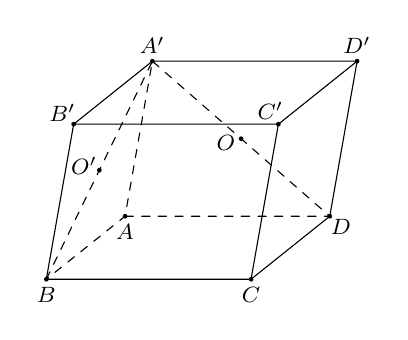
\begin{tikzpicture}[scale=1,>=stealth,font=\footnotesize,line join=round,line cap=round,declare function={h=2;}]
		 \path
			(0,0) coordinate  (A)
			(-1,-0.8) coordinate  (B)
			(1.6,-0.8) coordinate  (C)
			 (barycentric cs:A=1,C=1,B=-1) coordinate (D)
			(A)+(80:h) coordinate (A') 
			(barycentric cs:A=-1,B=1,A'=1) coordinate (B') 
			(barycentric  cs:A=-1,C=1,A'=1) coordinate (C')
			(barycentric cs:A=-1,D=1,A'=1) coordinate (D') 
			(barycentric cs:A'=1,D=1) coordinate  (O)
			(barycentric cs:A'=1,B=1) coordinate  (O');
		 \draw[dashed] (B)--(A')--(A)--(B)
			 (A)--(D)--(A');
		\draw (D')--(A')--(B')--(B)--(C)--(D)--(D')--(C')--(B') 
			(C)--(C'); 
		 \foreach \p/\g in{A/-90,B/-90,C/-90,D/-45,A'/90,B'/135,C'/120,D'/90,O/-165,O'/165}
		 \fill (\p) circle (.03) node[shift={(\g:.2)},scale=1]{$\p$};
	\end{tikzpicture}
	} 
	\choice 
		 {\True $OO'\perp AC$}
		{$OO'\perp AA'$} 
		 {$OO'\perp AD$}
		{$OO'\perp  AB$}
	\loigiai{ 
		\begin{center}
			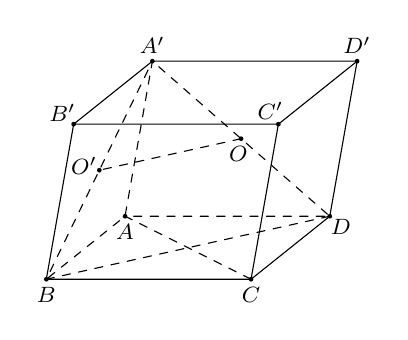
\begin{tikzpicture}[scale=1,>=stealth,font=\footnotesize,line join=round,line cap=round,declare function={h=2;}]
					\path 
						(0,0) coordinate  (A)
						(-1,-0.8) coordinate  (B)
						(1.6,-0.8)  coordinate (C)
						(barycentric cs:A=1,C=1,B=-1) coordinate (D) 
						 (A)+(80:h) coordinate (A')
						(barycentric cs:A=-1,B=1,A'=1) coordinate  (B')
						(barycentric cs:A=-1,C=1,A'=1)  coordinate (C')
						(barycentric  cs:A=-1,D=1,A'=1) coordinate (D')
						(barycentric cs:A'=1,D=1)  coordinate (O)
						(barycentric cs:A'=1,B=1)  coordinate (O');
					\draw[dashed] (D)--(B)--(A')--(A)--(B) 
						(C)--(A)--(D)--(A') 
						 (O)--(O');
					\draw  (D')--(A')--(B')--(B)--(C)--(D)--(D')--(C')--(B')
						 (C)--(C');
					\foreach \p/\g in{A/-90,B/-90,C/-90,D/-45,A'/90,B'/135,C'/120,D'/90,O/-100,O'/165} 
					 \fill (\p) circle (.03) node[shift={(\g:.2)},scale=1]{$\p$};
				\end{tikzpicture}
		\end{center}
		Ta có $\heva{&  OO'\parallel BD\\ & AC\perp BD}\Rightarrow OO'\perp AC$.
	 }
\end{ex}

% nguồn: Ok_Toan11_TracNghiem_Lan2
\begin{ex}%[1H8H2-3]%[ma:eb25d79f]
	Cho lăng trụ tam giác $ ABC.A'B'C'$ có đáy là tam giác đều.  Gọi $ M$ là trung điểm $ BC$. Khẳng định nào dưới đây đúng?
	 \choice
		{$AM\perp  A'B'$}
		 {$AM\perp BB'$}
		{\True  $AM\perp B'C'$}
		{$AM\perp  A'C'$}
	\loigiai{ 
	 \immini{
		 Do $ ABC$ là tam giác đều nên $ AM\perp BC$.\\
		Ta có $\heva{&AM\perp  BC\\ &BC\parallel B'C'}\Rightarrow AM\perp B'C'$.}
		{\begin{tikzpicture}[scale=1,font=\footnotesize,line join=round,line cap=round,>=stealth]
		\path 
			 (0,0) coordinate (A')
			 (2,-1.5) coordinate (B')
			(5,0) coordinate  (C')
			(-0.5,-3)  coordinate (A)
			($(A)+(B')-(A')$) coordinate  (B)
			 ($(B)+(C')-(B')$) coordinate (C)
			($(B)!0.5!(C)$)  coordinate (M);
		 \draw
			 (A')--(B')--(C')--cycle
			(A')--(A)--(B)--(B') 
			(B)--(C)--(C'); 
		 \draw[dashed]
			 (M)--(A)--(C);
		\foreach \p/\g  in {A'/170,B'/-30,C'/10,A/180,B/-45,C/0,M/-30}
		\draw[fill=black] (\p) circle (1pt) node[shift=(\g:3mm)] {$\p$}; 
		 \pic[draw,angle radius=6pt]{right angle=A--M--B};
	\end{tikzpicture}
		 }
	 }
\end{ex}

% nguồn: Ok_Toan11_TracNghiem_Lan2
\begin{ex}%[1H8H2-3]%[ma:66953f27]
	Cho hình hộp $ABCD.A'B'C'D'\,$ có tất cả các cạnh đều bằng nhau. Chọn khẳng định \textbf{sai} trong các khẳng định  sau.
	\choice 
		{\True $ AC\perp B'C'$} 
		 {$ BD\perp A'C'$}
		{$  AD'\perp CB'$}
		{$ AB'\perp  CD'$}
	\loigiai{ 
	 \immini{
		Hình  hộp $ABCD.A'B'C'D'$ có các mặt đều là hình thoi nên
		\begin{itemize}
			\item $BD\perp AC$, mà $AC\parallel A'C'$, suy ra  $BD\perp A'C'$.
			\item $AD'\perp A'D$, mà $A'D\parallel CB'$, suy ra $AD'\perp  CB'$.
			\item $AB'\perp A'B$, mà  $A'B\parallel CD'$, suy ra $AB'\perp CD'$.
		\end{itemize}
		Khẳng định sai là $ AC\perp B'C'$. 
		} 
		{\begin{tikzpicture}[scale=1,font=\footnotesize,line join=round,line cap=round,>=stealth]
		 \path
			(0,0)  coordinate (A)
			(1.5,1) coordinate  (B)
			(3,0) coordinate  (D)
			($(B)+(D)-(A)$) coordinate (C) 
			(0.5,3) coordinate (A') 
			($(A')+(B)-(A)$)  coordinate (B')
			($(B')+(C)-(B)$) coordinate  (C')
			($(A')+(D)-(A)$) coordinate (D'); 
		\draw 
			(A)--(A')--(D')--(D)--cycle 
			(A')--(B')--(C')--(C)--(D) 
			 (D')--(C')
			 (A')--(C');
		\draw[dashed] 
			 (A)--(B)--(C)
			(B')--(B) 
			(A)--(C); 
		 \foreach \p/\g in {A/170,B/170,C/10,D/-10,A'/180,B'/135,C'/0,D'/-30}
		 \draw[fill=black] (\p) circle (1pt) node[shift=(\g:3mm)] {$\p$};
	\end{tikzpicture}
		 }
	 }
\end{ex}

% nguồn: Ok_Toan11_TracNghiem_Lan2
\begin{ex}%[1H8H2-3]%[ma:7f8c5dc6]
	Cho hình chóp tam giác $S.ABC$ có $SA\perp\left(ABC\right)$, tam giác  $ ABC$vuông tại $ B$. Gọi $ H$là hình chiếu của $ A$ trên $ SB$. Xét các khẳng định sau\\
	 $(1).\,AH\perp SC;\quad\quad(2).\, BC\perp\left(SAB\right);\quad\quad (3).\, SC\perp AB$.\\
	Có bao nhiêu khẳng định  đúng?
	\choice 
		 {$3\cdot $}
		{$1\cdot $} 
		 {$0\cdot $}
		{\True  $2\cdot $}
	 \loigiai{
	\immini{ 
		Ta có  $\heva{&BC\perp AB\\&BC\perp SA}\Rightarrow BC\perp\left(SAB\right)\Rightarrow BC\perp AH$.\\
		Mặt khác $\heva{&AH\perp SB\\&BC\perp  AH}\Rightarrow AH\perp\left(SBC\right)\Rightarrow AH\perp SC$.}
		{\begin{tikzpicture}[scale=1,font=\footnotesize,line join=round,line cap=round,>=stealth]
		 \path
			(0,0) coordinate  (A)
			(1.5,-1.5) coordinate (B) 
			(4,0) coordinate (C) 
			(0,3) coordinate  (S)
			($(S)!0.55!(B)$) coordinate  (H);
		 \draw
			 (S)--(A)--(B)--(C)--(S)--(B)
			(A)--(H); 
		\draw[dashed] 
			 (A)--(C);
		 \foreach \p/\g in {A/180,B/-90,C/0,S/90,H/30}
		\draw[fill=black] (\p) circle (1pt) node[shift=(\g:3mm)]  {$\p$};
		\pic[draw,angle  radius=2mm]{right angle=A--H--B};
		 \pic[draw,angle radius=2mm]{right angle=A--B--C};
		\pic[draw,angle  radius=2mm]{right angle=S--A--C};
	\end{tikzpicture}
		} 
	} 
\end{ex}

% nguồn: Ok_Toan11_TracNghiem_Lan2
\begin{ex}%[1H8H2-3]%[ma:c356d597]
	Cho hình hộp $ABCD.A'B'C'D'$ có đáy là hình thoi. Gọi $(P)$ là mặt phẳng chứa $ A'C'$ và cắt $ AB$, $BC$ lần lượt tại $ I$ và $ J$. Trong các mệnh đề sau, mệnh đề nào  đúng?
	 \choice
		{$BD\perp  A'I$}
		{\True $BD\perp IJ$} 
		 {$BD\perp C'J$}
		 {$BD\perp A'J$}
	\loigiai{ 
	\immini{ 
		 Ta có $\heva{&(P)\cap\left(ABCD\right)=IJ\\ &(P)\cap\left(A'B'C'D'\right)=A'C'\\ &\left(ABCD\right)\parallel \left(A'B'C'D'\right)}\Rightarrow A'C'\parallel IJ$.\\
		Mà $ A'C'\parallel AC$ nên  $ IJ\parallel AC$.\\
		Mặt khác $\heva{&BD\perp AC\\ &AC\parallel IJ}\Rightarrow BD\perp IJ$.} 
		{\begin{tikzpicture}[scale=1,font=\footnotesize,line join=round,line cap=round,>=stealth]
		\path 
			(0,0) coordinate  (A)
			 (1.5,1) coordinate (B)
			 (3,0) coordinate (D)
			 ($(B)+(D)-(A)$) coordinate (C)
			(0.5,3) coordinate  (A')
			 ($(A')+(B)-(A)$) coordinate (B')
			 ($(B')+(C)-(B)$) coordinate (C')
			 ($(A')+(D)-(A)$) coordinate (D')
			($(B)!0.5!(A)$) coordinate (I) 
			 ($(B)!0.5!(C)$) coordinate (J);
		 \draw
			 (A)--(A')--(D')--(D)--cycle
			(A')--(B')--(C')--(C)--(D) 
			 (D')--(C')--(A');
		\draw[dashed] 
			(A)--(B)--(C)--cycle  (B')--(B)--(D)
			(A')--(I)--(J)--(C'); 
		\foreach \p/\g  in {A/170,B/170,C/10,D/-10,A'/180,B'/135,C'/0,D'/-30,I/170,J/110}
		\draw[fill=black] (\p)  circle (1pt) node[shift=(\g:3mm)] {$\p$};
	\end{tikzpicture}
		} 
	} 
\end{ex}

% nguồn: Ok_Toan11_TracNghiem_Lan2
\begin{ex}%[1H8H2-3]%[ma:b02e31dc]
	Cho tứ diện $OABC$ có $ OA$, $OB$, $OC$ đôi  một vuông góc. Đường thẳng $ OA$ vuông góc với đường thẳng nào sau đây?
	\choice 
		 {\True $ BC$}
		{$ AB$} 
		{$ AC$} 
		{$  OA$}
	\loigiai{ 
	\immini{ 
		Ta có $\heva{&OA\perp OB\\ &OA\perp OC}\Rightarrow OA\perp\left(OBC\right)\Rightarrow  OA\perp BC$.}
		{\begin{tikzpicture}[scale=1,font=\footnotesize,line join=round,line cap=round,>=stealth]
		 \path
			 (0,0) coordinate (O)
			 (-1.5,-1.5) coordinate (C)
			(4,0)  coordinate (B)
			 (0,3) coordinate (A);
		 \draw
			 (A)--(B)--(C)--cycle;
		\draw[dashed] 
			 (A)--(O)--(B)
			 (O)--(C);
		\foreach \p/\g in {A/20,B/10,C/170,O/-60} 
		\draw[fill=black] (\p)  circle (1pt) node[shift=(\g:3mm)] {$\p$};
		\pic[draw,angle  radius=2mm]{right angle=A--O--B};
		 \pic[draw,angle radius=2mm]{right angle=A--O--C};
		 \pic[draw,angle radius=2mm]{right angle=C--O--B};
	\end{tikzpicture}
		 }
	} 
\end{ex}

% nguồn: Ok_Toan11_TracNghiem_Lan2
\begin{ex}%[1H8H2-3]%[ma:96069b5a]
	Cho hình chóp $ S.ABCD$ có đáy $ ABCD$ là hình chữ nhật, $  SA\perp\left(ABCD\right)$. Biểu thức nào sau đây đúng?
	\choice 
		{$  SD\perp SB$}
		{$  BD\perp SC$}
		{$ SC\perp SB$} 
		 {\True $ SD\perp CD$}
	 \loigiai{
	\immini{ 
		Ta có $\heva{&SA\perp CD\\&AD\perp CD\\&SA\cap  AD=A}\Rightarrow CD\perp\left(SAD\right)\Rightarrow CD\perp SD$.}
		{\begin{tikzpicture}[scale=1,font=\footnotesize,line join=round,line cap=round,>=stealth]
		 \path
			 (0,0) coordinate (A)
			 (-1.5,-1.5) coordinate (B)
			 (4,0) coordinate (D)
			($(B)+(D)-(A)$) coordinate  (C)
			(0,3) coordinate (S); 
		\draw 
			(S)--(B)--(C)--(D)--(S)--(C); 
		 \draw[dashed]
			 (S)--(A)
			(B)--(A)--(D); 
		\foreach \p/\g in {A/170,B/-90,C/-90,D/0,S/90} 
		\draw[fill=black]  (\p) circle (1pt) node[shift=(\g:3mm)] {$\p$};
		 \pic[draw,angle radius=2mm]{right angle=S--A--D};
	\end{tikzpicture}
		} 
	 }
\end{ex}

% nguồn: Ok_Toan11_TracNghiem_Lan2
\begin{ex}%[1H8H2-3]%[ma:24d5ab57]
	 Cho hình chóp $ S.ABCD$ có $ SA\perp\left(ABCD\right)$. Tìm mệnh đề \textbf{sai} trong các mệnh đề dưới đây.
	 \choice
		{\True $  SA\perp SB$}
		{$  SA\perp CD$}
		{$ SA\perp BD$} 
		{$ SA\perp BC$} 
	 \loigiai{
	\immini{ 
		Ta có $ SA\perp\left(ABCD\right)$ nên $ SA\perp CD$, $ SA\perp BD$ và $ SA\perp BC$.}{\begin{tikzpicture}[scale=1,font=\footnotesize,line join=round,line cap=round,>=stealth]
		 \path
			(0,0)  coordinate (A)
			(-1.5,-1.5) coordinate  (B)
			(4,0) coordinate (D) 
			($(B)+(D)-(A)$) coordinate (C) 
			(0,3) coordinate (S); 
		 \draw
			(S)--(B)--(C)--(D)--(S)--(C); 
		 \draw[dashed]
			 (S)--(A)
			 (B)--(A)--(D);
		\foreach \p/\g in  {A/170,B/-90,C/-90,D/0,S/90}
		\draw[fill=black] (\p) circle (1pt)  node[shift=(\g:3mm)] {$\p$};
		\pic[draw,angle radius=2mm]{right  angle=S--A--D};
	\end{tikzpicture}
		} 
	 }
\end{ex}

% nguồn: Ok_Toan11_TracNghiem_Lan2
\begin{ex}%[1H8H2-3]%[ma:abb97939]
	 Cho hình chóp $ S.ABCD$ có đáy $ ABCD$ là hình chữ nhật. Gọi $M$, $N$ lần lượt là trung điểm của $ SC$ và $ SD$. Khẳng định nào dưới đây đúng?
	 \choice
		{$ MN\perp AC$} 
		{$  MN\perp BD$}
		{$  MN\perp AB$}
		{\True $ MN\perp  BC$}
	 \loigiai{
	 \immini{
		Ta có $MN$ là đường trung bình của tam giác $SCD$. Suy ra $MN \parallel  CD$.\\
		 Ta có $\heva{&MN\parallel CD\\ &BC\perp CD}\Rightarrow MN\perp BC$.}
		{\begin{tikzpicture}[scale=1,font=\footnotesize,line join=round,line cap=round,>=stealth]
		 \path
			(0,0) coordinate (A) 
			(-1.5,-1.5) coordinate (B) 
			(4,0) coordinate (D) 
			 ($(B)+(D)-(A)$) coordinate (C)
			 (0,3) coordinate (S)
			($(S)!0.5!(C)$)  coordinate (M)
			($(S)!0.5!(D)$)  coordinate (N);
		 \draw
			 (S)--(B)--(C)--(D)--(S)--(C)
			 (M)--(N);
		\draw[dashed] 
			 (S)--(A)
			(B)--(A)--(D); 
		\foreach \p/\g in {A/170,B/-90,C/-90,D/0,S/90,M/190,N/60} 
		\draw[fill=black] (\p)  circle (1pt) node[shift=(\g:3mm)] {$\p$};
	\end{tikzpicture}
		} 
	 }
\end{ex}

% nguồn: Ok_Toan11_TracNghiem_Lan2
\begin{ex}%[1H8H2-3]%[ma:ac22eb6d]
	Cho hình chóp $ S.ABCD$ có đáy $ ABCD$ là hình thoi tâm $ O$. Gọi  $I$, $J$ lần lượt là trung điểm của $ SA$ và $ SC$. Khẳng định nào dưới đây đúng?
	\choice 
		 {$ IJ\perp AB$}
		 {$ IJ\perp AD$}
		{\True $ IJ\perp  BD$}
		{$ IJ\perp SD$} 
	 \loigiai{
	 \immini{
		Vì $ IJ$ là đường trung bình của tam giác $ SAC$ nên  $ IJ\parallel AC$.\\
		Ta có $\heva{&IJ\parallel AC\\	&BD\perp AC}\Rightarrow BD\perp IJ$.}{\begin{tikzpicture}[scale=1,font=\footnotesize,line join=round,line cap=round,>=stealth]
		 \path
			(0,0)  coordinate (A)
			 (-1.5,-1.5) coordinate (B)
			(4,0) coordinate  (D)
			($(B)+(D)-(A)$)  coordinate (C)
			(0,3) coordinate  (S)
			($(S)!0.5!(A)$)  coordinate (I)
			($(S)!0.5!(C)$) coordinate  (J)
			 ($(C)!0.5!(A)$) coordinate (O);
		\draw 
			(S)--(B)--(C)--(D)--(S)--(C); 
		\draw[dashed] 
			 (S)--(A)--(C)
			 (B)--(A)--(D)--cycle (I)--(J);
		\foreach \p/\g  in {A/170,B/-90,C/-90,D/0,S/90,I/60,J/30,O/-90}
		 \draw[fill=black] (\p) circle (1pt) node[shift=(\g:3mm)] {$\p$};
		\pic[draw,angle radius=2mm]{right angle=A--O--B}; 
	\end{tikzpicture}
		} 
	 }
\end{ex}

% nguồn: Ok_Toan11_TracNghiem_Lan2
\begin{ex}%[1H8H2-3]%[ma:b2c53bb1]
	Cho hình chóp $ S.ABCD$ có đáy $  ABCD$ là hình bình hành tâm $ O$. Mặt bên $ SAB$ là tam giác cân. Gọi $ E$, $F$ lần lượt là trung điểm $ AB$và $ CD$. Khẳng định nào dưới đây \textbf{sai}?
	 \choice
		{$CD\perp SF$} 
		{\True  $CD\perp SE$}
		{$CD\perp SO$} 
		{$CD\perp EF$} 
	 \loigiai{
	\immini{ 
		Vì tam giác $ SAB$  cân tại $ S$ nên $ SE\perp AB$.\\
		Ta  có $\heva{&AB\parallel CD\\ &SE\perp AB}\Rightarrow CD\perp SE$.}
		{\begin{tikzpicture}[scale=1,font=\footnotesize,line join=round,line cap=round,>=stealth]
		 \path
			(0,0) coordinate (A) 
			(-1.5,-1.5) coordinate (B) 
			(4,0) coordinate  (D)
			($(B)+(D)-(A)$) coordinate  (C)
			(0,3) coordinate  (S)
			 ($(B)!0.5!(A)$) coordinate (E)
			($(C)!0.5!(D)$) coordinate  (F)
			 ($(C)!0.5!(A)$) coordinate (O);
		 \draw
			(S)--(B)--(C)--(D)--(S)--(C) 
			(S)--(F); 
		 \draw[dashed]
			 (S)--(A)
			(B)--(A)--(D) 
			 (O)--(S)--(E)--(F);
		\foreach \p/\g in {A/160,B/-90,C/-90,D/0,S/90,E/170,F/-20,O/-90} 
		\draw[fill=black] (\p) circle (1pt)  node[shift=(\g:3mm)] {$\p$};
	\end{tikzpicture}
		 }
	} 
\end{ex}

% nguồn: Ok_Toan11_TracNghiem_Lan2
\begin{ex}%[1H8H2-3]%[ma:bb6d2275]
	Cho hình chóp $ S.ABC$  có $ SA\perp\left(ABC\right)$ và $ H$ là hình chiếu vuông góc của S lên $ BC$. Hãy chọn khẳng định đúng.
	\choice 
		{$ BC\perp  AB$}
		 {$ BC\perp AC$}
		 {$ BC\perp SC$}
		 {\True $ BC\perp AH$}
	\loigiai{ 
	\immini{ 
		Ta có $\heva{&SA\perp BC\\&SH\perp BC}\Rightarrow AH\perp  BC$.}
		{\begin{tikzpicture}[scale=1,font=\footnotesize,line join=round,line cap=round,>=stealth]
		 \path
			(0,0) coordinate  (A)
			(1.5,-1.5)  coordinate (B)
			(4,0) coordinate (C) 
			 (0,3) coordinate (S)
			($(B)!0.4!(C)$) coordinate  (H);
		\draw 
			(S)--(A)--(B)--(C)--(S)--(B) 
			(S)--(H); 
		 \draw[dashed]
			 (H)--(A)--(C);
		\foreach \p/\g  in {A/180,B/-90,C/0,S/90,H/-30}
		\draw[fill=black] (\p) circle  (1pt) node[shift=(\g:3mm)] {$\p$};
		\pic[draw,angle radius=6pt]{right  angle=S--H--C};
		 \pic[draw,angle radius=2mm]{right angle=S--A--C};
	\end{tikzpicture}
		} 
	} 
\end{ex}

% nguồn: Ok_Toan11_TracNghiem_Lan2
\begin{ex}%[1H8H2-3]%[ma:917bbf9e]
	Cho hình chóp $S.ABC$ có  $ SA\perp\left(ABC\right)$ và tam giác $ ABC$ vuông ở $ B$, $ AH$ là đường cao của tam giác $ SAB$. Khẳng định nào sau đây là khẳng định \textbf{sai}?
	 \choice
		{$  SA\perp BC$}
		 {\True $ AH\perp AC$}
		{$ AH\perp  SC$}
		{$  AH\perp BC$}
	 \loigiai{
	\immini{ 
		$ SA\perp\left(ABC\right)\Rightarrow SA\perp BC$ suy ra phương án $ SA\perp BC$ đúng.\\ 
		Ta có $\heva{&BC\perp  AB~\left(\triangle ABC \text{ vuông tại }B\right)\\&BC\perp SA~\left(\text{do } SA\perp\left(ABC\right)\right)}\\
		\Rightarrow BC\perp\left(SAB\right)\Rightarrow BC\perp  AH$.\hfill$(1)$\\
		 Lại có $ AH\perp SB$.\hfill$(2)$\\
		Từ $(1)$ và  $(2)$ suy ra $AH\perp\left(SBC\right)\Rightarrow AH\perp SC$, $AH\perp BC$.\\
		Suy ra phương án $ AH\perp SC$, $ AH\perp BC$ đúng.} 
		{\begin{tikzpicture}[scale=1,font=\footnotesize,line join=round,line cap=round,>=stealth]
		 \path
			(0,0) coordinate (A) 
			(1.5,-1.5) coordinate (B) 
			 (4,0) coordinate (C)
			 (0,3) coordinate (S)
			($(S)!0.55!(B)$) coordinate  (H);
		\draw 
			(S)--(A)--(B)--(C)--(S)--(B) 
			(A)--(H); 
		 \draw[dashed]
			 (A)--(C);
		\foreach \p/\g in {A/180,B/-90,C/0,S/90,H/30} 
		\draw[fill=black]  (\p) circle (1pt) node[shift=(\g:3mm)] {$\p$};
		 \pic[draw,angle radius=2mm]{right angle=A--H--B};
		 \pic[draw,angle radius=2mm]{right angle=A--B--C};
		\pic[draw,angle radius=2mm]{right  angle=S--A--C};
	\end{tikzpicture}
		} 
	 }
\end{ex}

% nguồn: Ok_Toan11_TracNghiem_Lan2
\begin{ex}%[1H8H2-3]%[ma:6afd536d]
	Cho hình chóp $S.ABC$ có $SA\perp  (ABC)$ và $AB\perp BC$ . Hình chóp $SABC$ có bao nhiêu mặt là tam giác vuông?
	 \choice
		{$  2$}
		{\True $  4$}
		 {$ 3$}
		{$  1$}
	 \loigiai{
	\immini{ 
		Ta có $SA\perp (ABC)$ nên $SA\perp AB$, suy ra tam giác $SAB$  vuông tại $A$.\\
		Lại có $SA\perp (ABC)$ nên $SA\perp AC$, suy  ra tam giác $SAC$ vuông tại $A$.\\
		Vì $AB\perp BC$ nên $\triangle ABC$ là tam giác vuông.\\ 
		Ta lại có $\heva{&{BC\perp SA}\\&BC\perp AB}\Rightarrow BC\perp (SAB)$.\\ 
		$\Rightarrow BC\perp SB$ nên tam giác $SBC$ là tam giác vuông  tại $B$.\\
		Vậy hình chóp $S.ABC$ có bốn  mặt là tam giác vuông.}
		{\begin{tikzpicture}[scale=1,font=\footnotesize,line join=round,line cap=round,>=stealth]
		\path 
			(0,0)  coordinate (A)
			 (1.5,-1.5) coordinate (B)
			 (4,0) coordinate (C)
			(0,3) coordinate (S); 
		 \draw
			 (S)--(A)--(B)--(C)--(S)--(B);
		\draw[dashed] 
			(A)--(C); 
		\foreach \p/\g  in {A/180,B/-90,C/0,S/90}
		\draw[fill=black] (\p) circle  (1pt) node[shift=(\g:3mm)] {$\p$};
		\pic[draw,angle radius=2mm]{right angle=S--A--C}; 
		\pic[draw,angle radius=2mm]{right angle=A--B--C}; 
	\end{tikzpicture}
		 }
	} 
\end{ex}

% nguồn: Ok_TracNghiemLop11_Lan1
\begin{ex}%[1H8H2-3]%[ma:9683e0fd]
	Cho tứ  diện $ABCD$ có $\triangle ABC$ và $\triangle DBC$ là hai tam giác đều. Gọi $I$ là trung điểm của $BC$, $AH$ là đường cao của tam giác $AID$. Đường thẳng $BC$ không vuông góc với đường thẳng nào sau đây?
	 \choice
		 {\True $AC$}
		 {$AH$}
		 {$AD$}
		 {$AI$}
	\loigiai{ 
	\immini{ 
		 Ta có $\triangle ABC$ đều nên $\widehat{ACB}=60^\circ$.\\
		Suy  ra $BC\perp AC$ là khẳng định sai.
		 }
		{ 
		\begin{tikzpicture}
				 \def\a{3}
				\path (0:0) coordinate (B) 
					++(0:\a)  coordinate (D)
					++(-120:\a/2) coordinate  (C)
					($(B)+(70:\a)$) coordinate (A) 
					($(B)!.5!(C)$) coordinate  (I)
					($(D)!.7!(I)$)  coordinate (H);
				 \draw[dashed] (B)--(D)--(I)
					 (A)--(H);
				 \draw (B)--(A)--(D)
					(I)--(A)--(C) 
					(B)--(C)--(D); 
				 \foreach \x/\g in {A/90,B/180,C/-45,D/0,H/-60,I/-90}
				 \fill[black] (\x) circle (1pt)
					 ($(\g:3mm)+(\x)$) node {$\x$};
			\end{tikzpicture}
		 }
	 }
\end{ex}

% nguồn: Ok_TracNghiemLop11_Lan1
\begin{ex}%[1H8H2-3]%[ma:b6a8be76]
	Cho hình chóp $S.ABC$ có $SA=SB=SC=a$, $\widehat{ASB}=\widehat{BSC}$. Khẳng định nào  sau đây là đúng?
	 \choice
		 {$SA\perp BC$}
		{$SC\perp  AB$}
		{\True $SB\perp  AC$}
		 {$SA\perp SC$}
	\loigiai{ 
		 \allowdisplaybreaks
		Ta có 
		\begin{eqnarray*}
			\overrightarrow{SB}\cdot\overrightarrow{AC} 
			 &=&\overrightarrow{SB}\left(\overrightarrow{SC}-\overrightarrow{SA}\right)\\
			 &=&\overrightarrow{SB}\cdot\overrightarrow{SC}-\overrightarrow{SB}\cdot\overrightarrow{SA}\\
			&=&SB\cdot SC\cdot\cos\widehat{BSC}-SB\cdot  SA\cdot\cos\widehat{ASB}\\
			 &=&SA^2\cdot\left(\cos \widehat{BSC}-\cos \widehat{ASB}\right)\\
			 &=&0
		\end{eqnarray*}
		 $\Rightarrow$$SB\perp AC$
	 }
\end{ex}

% nguồn: Ok_TracNghiemLop11_Lan1
\begin{ex}%[1H8H2-3]%[ma:458f91c2]
	Cho hình chóp $S.ABC$ có $SA$ vuông góc với mặt phẳng $(ABC)$ và đáy $ABC$ là tam giác cân tại $C$. Gọi $H$ và $K$  lần lượt là trung điểm của $AB$ và $SB$. Khẳng định nào sau đây là \textbf{sai}?
	 \choice
		 {$CH\perp SB$}
		{$CH\perp  SA$}
		{$CH\perp  AK$}
		{\True  $AK\perp BC$}
	\loigiai{ 
		 Ta có $\heva{&SA\perp (ABC)\\&CH \subset (ABC)} \Rightarrow SA \perp CH$.\\
		 Do $\heva{& CH \perp SA\\&CH \perp AB }$ nên
		$CH\perp  (SAB)$.\\
		Từ đó $CH\perp SB$ và  $CH\perp AK \subset (SAB)$.
	 \immini{
		Nếu $AK\perp BC$ là đúng thì $\heva{&  AK \perp BC\\& AK \perp CH.}$ \\
		Suy ra $AK \perp (ABC) \Rightarrow AK \perp AB  \Rightarrow S,A,K$ thẳng hàng (vô lý).\\
		 Vậy chắc chắn $AK\perp BC$ là sai.
		} 
		{\begin{tikzpicture}[line width=0.6pt,line cap=round,line join=round,>=stealth,scale=1]
		\coordinate[label=left:{$A$}] (A)  at (0,0);
		\coordinate[label=below:{$B$}] (B)  at (1.5,-1);
		\coordinate[label=right:{$C$}]  (C) at (4,0);
		\coordinate[label=below left:{$H$}]  (H) at ($(B)!0.5!(A)$);
		 \coordinate[label={$S$}] (S) at ($(A)+(0,3)$);
		\coordinate[label=right:{$K$}] (K) at ($(B)!0.5!(S)$); 
		\draw (S)--(B)--(C)--(S)--(A)--(B) 
			(A)--(K); 
		\draw[dashed]  (A)--(C)--(H);
		\foreach \x/\dinh/\y in {C/H/B,S/A/B}  \draw[fill = gray!50] ($(\dinh)!3pt!(\x)$)--($(\dinh)!3pt!(\x)+(\dinh)!3pt!(\y)-(\dinh)$)--($(\dinh)!3pt!(\y)$)--(\dinh)--cycle;
		\foreach \p in {A,B,C,H,S,K} 
		\fill (\p) circle  (1pt);
	\end{tikzpicture}
	 }}
\end{ex}

% nguồn: Ok_TracNghiemLop11_Lan1
\begin{ex}%[1H8H2-3]%[ma:15c5b791]
	Cho hình chóp $S. A B C D$ đáy $A B C D$  là hình bình hành, $S A$ vuông góc với mặt phẳng $(A B C D)$. Góc tạo bởi giữa hai đường thẳng nào sau đây bằng $90^{\circ}$?
	 \choice
		{$S A,  S B$}
		 {$S A, S C$}
		{\True $S A, B D$} 
		{$S B, A  D$}
	 \loigiai{
		\begin{center}
			\begin{tikzpicture}
					\def\a{3} 
					\def\h{3} 
					 \path (0:0) coordinate (A)
						 ++(0:\a) coordinate (D)
						++(-130:\a/2) coordinate (C) 
						 ($(A)+(C)-(D)$) coordinate (B)
						($(A)+(90:\h)$) coordinate (S) 
						(intersection of A--C and  B--D) coordinate (O);
					\draw[dashed]  (B)--(A)--(D)
						(A)--(S) 
						 (A)--(C)
						 (B)--(D);
					 \draw[thick] (B)-- (C)--(D)
						 (B)--(S)
						(C)--(S) 
						(D)--(S); 
					\foreach \x/\g in {A/135,B/-135,C/-45,D/45,S/90} 
					 \fill[black] (\x) circle (1pt)
						 ($(\g:3mm)+(\x)$) node {$\x$};
					 \draw pic[draw,angle radius=2mm]{right angle=D--A--S};
				\end{tikzpicture}
		\end{center}
		$ 
		 \heva{
		&S A \perp(A B  C D) \\
		&B D \subset(A  B C D)\\
		} \Rightarrow S A  \perp B D \Rightarrow(S A, B D)=90^{\circ}.
		 $
	} 
\end{ex}

% nguồn: Ok_TracNghiemLop11_Lan1
\begin{ex}%[1H8H2-3]%[ma:6ac67471]
	\immini 
	{ 
	Cho hình chóp $S.ABC$ có $SA\perp (ABC)$. $H$ là hình chiếu vuông góc của $S$ lên cạnh $BC$.  Hãy chọn khẳng định đúng.
	 \choice
		 {$BC\perp SC$}
		{$BC\perp  AB$}
		{$BC\perp  AC$}
		{\True $BC\perp  AH$}
		} 
		{ 
		\begin{tikzpicture}[scale=0.6,>=stealth,font=\footnotesize,line join=round,line cap=round]
				\coordinate  (A) at (-2,0);
				\coordinate (B) at  (0,-2);
				\coordinate  (C) at (3,0);
				\coordinate (S)  at ($(A)+(0,4)$);
				 \path
					($(B)!.4!(C)$)  coordinate (H);
				\draw  (S)--(A)
					 (S)--(B)
					 (H)--(S)--(C)
					 (B)--(C)
					(A)--(B); 
				 \draw[dashed](H)--(A)--(C);
				\pic[draw,angle radius=2mm] {right angle = S--A--B} pic[draw,angle radius=2mm]  {right angle = S--A--C};
				\foreach \i/\g in {S/90,A/180,B/-90,C/0,H/-90}{\draw[fill](\i) circle  (1pt)
					($(\i)+(\g:3mm)$)  node[scale=1]{$\i$};}
			\end{tikzpicture}
		 }
	 \loigiai{
		Ta có $\heva{&BC\perp SA\\&BC\perp SH}\Rightarrow BC\perp (SAH)\Rightarrow BC\perp AH$. 
	 }
\end{ex}

% nguồn: Ok_TracNghiemLop11_Lan1
\begin{ex}%[1H8H2-3]%[ma:b5ed1c7e]
	Cho tứ diện $MNPQ$ có hai tam giác $MNP$  và $QNP$ là hai tam giác cân lần lượt tại $M$ và $Q$. Góc giữa hai đường thẳng $MQ$ và $NP$ bằng
	\choice 
		{$45^{\circ}$} 
		{$30^{\circ}$} 
		{$60^{\circ}$} 
		{\True $90^{\circ}$} 
	\loigiai{ 
	\immini{Gọi $I$ là trung điểm của $NP$.\\ 
		Khi đó $\triangle{MNP}$ cân tại $M$  nên $NP \perp MI$.\\
		Tương tự $\triangle{QNP}$ cân tại $Q$ nên $NP  \perp QI$.\\
		Ta có $\heva{&NP \perp MI\\ &NP \perp QI} \Rightarrow NP \perp  (MQI) \Rightarrow NP \perp MQ$.\\
		Suy ra góc giữa hai đường  thẳng $MQ$ và $NP$ bằng $90^{\circ}$.}{
		\begin{tikzpicture}[line join=round,line cap=round,>=stealth,scale=0.7]
				\path 
					(0,0)  coordinate (N) node[left]{$N$}
					(2,-2) coordinate  (P) node[below]{$P$}
					(5,0) coordinate  (Q) node[right]{$Q$}
					(3,4) coordinate (M) node[above]{$M$}; 
				\coordinate[label=below left:$I$]  (I) at ($(N)!0.5!(P)$);
				\draw  (I)--(M)--(N)--(P)--(Q)--(M)--(P);
				\draw[dashed] (N)--(Q)--(I); 
				\draw pic[draw,angle  radius=2mm,angle eccentricity=1.5]{right angle = Q--I--P};
				\draw pic[draw,angle radius=2mm,angle eccentricity=1.5]{right angle =  M--I--N};
				 \foreach \i in {M,N,P,Q,I}{\draw[fill](\i) circle (1pt);}
			\end{tikzpicture}
		 }
	 }
\end{ex}

% nguồn: Ok_TracNghiemLop11_Lan1
\begin{ex}%[1H8H2-3]%[ma:1abfcd25]
	Cho hình chóp $S.ABC$ có tam giác $ABC$ nhọn, $SA\perp(ABC)$ và $H$ là hình chiếu vuông góc của $S$ lên $BC$ ($H$ không trùng với $B$,  $C$). Trong các khẳng định sau, khẳng định nào đúng?
	\choice 
		 {$BC \perp SC$}
		{\True  $BC \perp AH$}
		{$BC \perp  AB$}
		{$BC  \perp AC$}
	 \loigiai{
	\immini{ 
		 Ta có $BC\perp SH$.\\
		Do $SA\perp(ABC)\Rightarrow SA\perp BC$ nên suy ra $BC\perp(SAH) \Rightarrow BC\perp  AH$.
		}{ 
		\begin{tikzpicture}[scale=1,line join=round,line cap=round,>=stealth]
				\path 
					(0,0) coordinate  (A)
					(1,-1) coordinate (B) 
					(3,0) coordinate (C) 
					(0,3) coordinate  (S)
					 ($(B)!0.4!(C)$) coordinate (H);
				 \draw
					(S)--(A)--(B)--(C)--cycle 
					(B)--(S)--(H); 
				 \draw[dashed] (H)--(A)--(C);
				\draw  pic[draw,angle radius=2mm]{right angle=S--A--C};
				\draw pic[draw,angle radius=2mm]{right  angle=S--H--C};
				\foreach \x/\g in {A/180,B/-90,C/0,S/90,H/-60} \fill[black](\x) circle (1pt)+(\g:0.3)  node{$\x$};
			\end{tikzpicture}
		 }
	 }
\end{ex}

% nguồn: Ok_TracNghiemLop11_Lan1
\begin{ex}%[1H8H2-3]%[ma:b2e05827]
	Cho hình chóp $S.ABCD$  có $SA \perp(ABCD)$, $ABCD$ là hình vuông. Khẳng định nào sau đây \textbf{sai}?
	 \choice
		 {$SA \perp AD$}
		{$SB \perp BC$} 
		 {$SA \perp BC$}
		{\True $SB \perp AC$} 
	\loigiai{ 
	\immini{ 
		\begin{itemize}
			\item Vì $SA\perp (ABCD)$ nên $SA  \perp AD$, $SA \perp BC$.
			\item Ta  có $\heva{
			& BC\perp AB\quad\left( ABCD\,\text{là hình vuông}  \right) \\
			& BC\perp SA\quad\left(SA\perp (ABCD) \right)}$\\ 
			$\Rightarrow BC\perp (SAB)\Rightarrow  BC\perp SB$.
			\item Ta có $\heva{& S\notin AC\\& SA\perp AC}$  nên chỉ có đường thẳng $SA$ vuông góc với $AC$. Do đó không tồn tại $SB\perp AC$.
		\end{itemize}
		 }
		{\begin{tikzpicture}[font=\footnotesize,line join=round,line cap=round,>=stealth,scale=0.6]
		 \path
			(0,0) coordinate (A) 
			(-2,-2)  coordinate (B)
			(3,-2) coordinate (C) 
			(5,0)  coordinate (D)
			(0,4) coordinate  (S);
		 \draw
			 (S)--(B)--(C)--(D)--cycle
			(S)--(C); 
		 \draw [dashed] (S)--(A)--(D)
			 (B)--(A);
		\draw  pic[draw,angle radius=5,angle eccentricity=1.5]{right angle=S--A--D};
		\foreach  \x/\g in
			{A/150,B/180,C/0,D/0,S/90} 
		\fill[black](\x) circle (1pt) 
			 ($(\x)+(\g:3mm)$) node{$\x$};
	\end{tikzpicture}
		} 
	} 
\end{ex}

% nguồn: Ok_Toan11_TracNghiem_Lan2
\begin{ex}%[1H8V2-3]%[ma:3e464698]
	Cho hình chóp $S.ABC$ có đáy $ABC$ là tam giác vuông tại $B$, cạnh bên $SA$ vuông góc với đáy. Gọi $H$ là chân đường cao kẻ  từ $A$ của tam giác $SAB$. Khẳng định nào dưới đây là \textbf{\textcolor{violet}{sai}}?
	 \choice
		{$SA\perp BC$} 
		{$AH\perp BC$} 
		{\True $AH\perp  AC$}
		 {$AH\perp SC$}
	\loigiai{ 
		\begin{center}
			\begin{tikzpicture}[scale=1,>=stealth,font=\footnotesize,line join=round,line cap=round,declare function={h=2;}]
					 \path
						(0,0) coordinate (A) 
						(0.7,-0.6) coordinate  (B)
						(2.5,0) coordinate  (C)
						 (A)+(90:h) coordinate (S)
						 (barycentric cs:B=4,S=3) coordinate (H);
					\draw[dashed]  (A)--(C);
					\draw  (H)--(A)--(B)--(C)--(S)--(A)
						(S)--(B); 
					\pic[draw,angle radius=4]{right  angle=S--H--A};
					 \foreach \p/\g in{A/-135,B/-90,C/-90,S/90,H/30}
					 \fill (\p) circle (.03) node[shift={(\g:.23)},scale=1]{$\p$};
				\end{tikzpicture}
		\end{center}
		\begin{itemize}
			\item Do  $SA\perp(ABC)$ nên $SA\perp BC$ đúng.
			 \item Ta có $\heva{& BC\perp AB\\ & BC\perp SA~(\text{do}SA\perp(ABC))\\ & AB\cap SA=A\\ & AB,SA\subset(SAB)}\Rightarrow BC\perp(SAB)$.\\
			Mặt khác, $\heva{& AH\perp SB\\ &  AH\perp BC~(\text{do~}BC\perp(SAB))\\ & SB\cap BC=B\\ & SB,BC\subset(SBC)}\Rightarrow AH\perp(SBC)$. \hfill$(1)$\\
			Từ $(1)$ suy ra  $AH\perp BC$ đúng.
			\item Từ $(1)$ suy ra $AH\perp SC$  đúng.
			\item Nếu $AH\perp  AC$ thì kết hợp với $SA\perp AC$ ta suy ra $AC\perp(SAH)$.\\
			Mà $AB\subset(SAH)$ nên $AC\perp AB$ (Vô lý, vì tam giác $ABC$ vuông tại  $B$).\\
			Vậy $AH$ không vuông  góc với $AC$.
		\end{itemize}
	} 
\end{ex}


%%%%%%%%%%%%%%%% ĐÚNG/SAI %%%%%%%%%%%%%%%%

% nguồn: Ok_dungsai_lop11_Lan1
\begin{ex}%[1H8N2-3]%[ma:63ef34f3]
 Cho hình  chóp $S.ABCD$ có đáy là hình chữ nhật, $SA\bot (ABCD)$.
  \choiceTF
  {\True $(SA,CD)=90^{\circ}$} 
  {\True $DC\bot  (SAD)$}
   {$BD\bot AC$}
  {$BD\bot (SAC)$} 
 \loigiai{ 
 \immini{ 
  \begin{itemize}
   \item $SA\bot  (ABCD)\Rightarrow SA\bot CD$.
   \item Ta có $\heva{&DC\bot AD\\&DC\bot  SA}\Rightarrow DC\bot (SAD)$.
   \item Vì $ABCD$ là hình chữ nhật  nên $BD$ không vuông góc với $AC$.
   \item  $BD$ không vuông góc với mặt phẳng $(SAC)$.
  \end{itemize}
  } 
  { 
  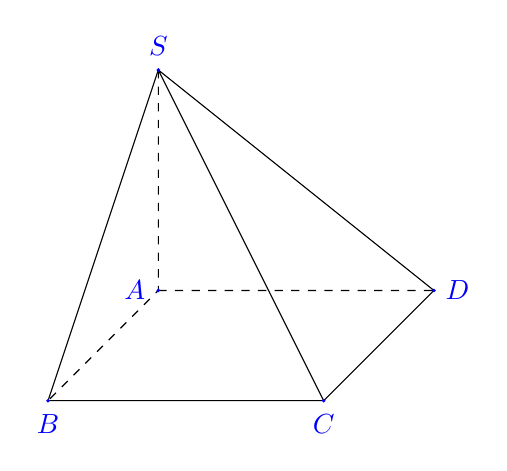
\begin{tikzpicture}[scale=0.7]
    \path  (0,0) coordinate (A)
     (-2,-2) coordinate  (B)
     (5,0) coordinate  (D)
     (3,-2) coordinate (C) 
      (0,4) coordinate (S);
    \draw[dashed] (S)--(A)--(B) 
      (A)--(D);
    \draw (B)--(C)--(D)--(S)--(B) 
     (S)--(C); 
    \foreach \p/\q  in {A/180,B/-90,C/-90,D/0,S/90}
    \fill[blue] (\p) circle (1pt) node[shift={(\q:3mm)}]{$\p$}; 
   \end{tikzpicture}
   }
 } 
\end{ex}

% nguồn: Ok_dungsai_lop11_Lan1
\begin{ex}%[1H8H2-3]%[ma:87df2400]
 Cho hình chóp  $S.ABC$ có đáy $ABC$ là tam giác cân tại $A$, cạnh bên $SA$ vuông góc với đáy, $M$ là trung điểm $BC$, $J$ là trung điểm $BM$. Xét tính Đúng/ Sai các khẳng định sau
  \choiceTF
  {$BC \perp  (SAB)$}
  {\True $BC  \perp (SAM)$}
   {\True $AM \perp BC$}
  {$BC \perp  (SAJ)$}
  \loigiai{
 \immini{ 
  Tam giác $ABC$ cân tại $A$  và $M$ là trung điểm của $BC$ nên $AM \perp BC$. \\
  Lại có $SA \perp (ABC)$  nên $SA \perp BC$.\\
  Trong $ (SAM)  $, $AM\cap SA=A$.\\
  Suy ra $BC  \perp (SAM)$.
   }{
  \begin{tikzpicture}[scale=.7,font=\footnotesize,line join=round,line cap=round,>=stealth]
     \path
      (0,0) coordinate (A)
     (2,-2) coordinate (B) 
     (5,0) coordinate  (C);
    \coordinate  (S) at ($(A)+(0,3)$);
    \coordinate (M)  at ($(C)!.5!(B)$);
    \coordinate (J)  at ($(B)!.5!(M)$);
     \draw (S)--(A)--(B)--(C)--cycle (M)--(S)--(B)
      (S)--(J);
    \draw[dashed] (M)--(A)--(C) 
      (A)--(J);
    \foreach \x/\g in {S/90,A/180,B/-90,C/0,M/-90,J/-90}\fill  (\x) circle (1pt)+(\g:0.25) node{$\x$};
     \path pic[draw,angle radius=5]{right angle=C--A--S};
   \end{tikzpicture}
  } 
  \begin{itemchoice}
    \itemch Sai
   \itemch  Đúng
   \itemch  Đúng
    \itemch Sai
  \end{itemchoice}
 } 
\end{ex}

% nguồn: Ok_dungsai_lop11_Lan1
\begin{ex}%[1H8H2-3]%[ma:1c7093ec]
 Cho hình chóp $S.ABCD$ có đáy là hình chữ nhật và $SA$ vuông góc với mặt phẳng đáy. Gọi $H$,  $K$ theo thứ tự là hình chiếu của $A$ trên các cạnh $SB$, $SD$. Khi đó
 \choiceTF 
  {\True Tam  giác $SBC$ vuông}
  {\True Tam giác $SCD$  vuông}
   {\True $SC \perp(AHK)$}
  {\True $HK \perp  SC$}
  \loigiai{
  \begin{center}
   \begin{tikzpicture}[scale=1,line cap=round,line join=round,font=\footnotesize,>=stealth]
     \path 
      (0,0)  coordinate (A)
       ($(A)+(-150:1.5)$) coordinate (B)
      ($(A)+(0:4)$) coordinate (D) 
       ($(B)+(0:4)$) coordinate (C)
      ($(A)+(90:3)$)  coordinate (S)
       ($(S)!0.4!(B)$) coordinate (H)
      ($(S)!0.4!(D)$) coordinate (K); 
     \draw  (S)--(B)--(C)--(D)--(S)--(C);
     \draw[dashed]  (S)--(A)--(B)
       (A)--(K)--(H)--(A)--(D);
     \foreach \p/\r in  {A/-60,B/-90,C/-90,D/0,H/150,K/20,S/90}
     \fill  (\p) circle (1.25pt) node[shift={(\r:3mm)}]{$\p$};
    \end{tikzpicture}
  \end{center}
  \begin{itemize}
   \item Ta có $\heva{&BC \perp AB \\& BC \perp SA (\text{do } SA \perp(ABCD))}  \Rightarrow BC \perp(SAB)$.\\
   Vì $\heva{&BC \perp(SAB) \\ &SB \subset(SAB)}\Rightarrow BC \perp SB$ hay $\triangle  SBC$ vuông tại $B$.
   \item Ta có $\heva{&CD \perp AD \\&CD \perp SA (\text {do } S A \perp(ABC D))} \Rightarrow  CD \perp(SAD)$.\\
   Vì $\heva{&CD  \perp(SAD) \\& SD \subset(SAD)}\Rightarrow CD \perp SD $ hay $\triangle SCD$ vuông tại $D$.
   \item Ta có $\heva{&AH \perp SB \\&AH \perp BC (\text {do } BC \perp(SA B))} \Rightarrow AH  \perp(SBC) \Rightarrow AH \perp SC$.\hfill (1)\\
   Tương tự $\heva{&AK \perp SD \\& AK \perp CD ~(\text {do } CD \perp(SA D))} \Rightarrow AK \perp(SCD)  \Rightarrow AK \perp SC$.\\
   Từ (1)  và (2) suy ra $SC \perp(AHK)$, mà $HK \subset(AHK)$ nên $HK \perp SC$.
  \end{itemize}
  }
\end{ex}

% nguồn: Ok_dungsai_lop11_Lan1
\begin{ex}%[1H8H2-3]%[ma:4950e91b]
 Cho tứ diện $OABC$ có $OA$, $OB$, $OC$ đôi một vuông góc với nhau. Gọi $OK$ là đường cao của tam giác $OBC$ và $OH$ là đường cao của tam giác $OAK$. Khi  đó
  \choiceTF
  {\True $OA\perp(OBC)$} 
   {\True $OA\perp(OBC)$, $OB\perp(OAC)$}
  {\True Các cạnh  đối nhau trong tứ diện $OABC$ thì vuông góc với nhau}
  {$OH$ không vuông góc với  mặt phẳng $(ABC)$}
  \loigiai{\immini{Ta có $\heva{&OA\perp OB\\&OA\perp OC}\Rightarrow OA\perp(OBC)$.\\
  $\heva{&OB\perp OA\\&OB\perp OC}\Rightarrow  OB\perp(OAC)$.\\
   Vì $OA\perp(OBC)$ mà $BC\subset(OBC)\Rightarrow OA\perp BC$.\\
  Vì $OB\perp(OAC)$ mà  $AC\subset(OAC)\Rightarrow OB\perp AC$.\\
  Ta  có: $\heva{&OC\perp OA\\&OC\perp OB}\Rightarrow OC\perp(OAB)$.\\
  Mà  $AB\subset(OAB)\Rightarrow OC\perp AB$.}
  {\begin{tikzpicture}[>=stealth,line join=round,line cap=round,font=\footnotesize,scale=0.65]
  \path (0,0) coordinate (O) 
   (0,5) coordinate  (A)
   (-2,-1.4) coordinate  (B)
   (6,0) coordinate  (C)
    ($(B)!0.45!(C)$) coordinate (K)
   ($(A)!0.7!(K)$)  coordinate (H);
  \draw (A)--(B)--(C)--(A)--(K); 
  \draw[dashed] (A)--(O)--(B) 
    (O)--(C)
   (H)--(O)--(K); 
  \foreach \p / \r in {B/-135,C/45,O/135,A/90,K/-45,H/45} 
  \fill (\p) circle  (1.2pt) node[shift={(\r:2.5mm)}]{$\p$};
  \pic[draw,angle radius=2mm,angle eccentricity=1.5] {right angle = O--H--K}; 
  \pic[draw,angle  radius=2mm,angle eccentricity=1.5] {right angle = A--O--C};
  \pic[draw,angle radius=2mm,angle eccentricity=1.5] {right  angle = B--O--C};
 \end{tikzpicture}
   }
   \noindent
  Vậy các cặp cạnh đối nhau  của tứ diện $OABC$ vuông góc với nhau.\\
  Ta có $\heva{&BC\perp OK\\&BC\perp  OA(\text{ do }OA\perp(OBC))}\Rightarrow BC\perp(OAK)$.\\
  mà $OH\subset(OAK)\Rightarrow OH\perp BC$.\\ 
  Khi đó $\heva{&OH\perp AK\\&OH\perp BC\\&AK\cap BC=K\\&AK, BC\subset(ABC)}\Rightarrow OH\perp(ABC)$.}
\end{ex}

% nguồn: Ok_dungsai_lop11_Lan1
\begin{ex}%[1H8H2-3]%[ma:b18722be]
 Cho tứ diện $A B C D$ có $A B=A C=A D=1$ và $\widehat{B A C}=\widehat{BAD}=60^{\circ}, \widehat{CAD}=90^{\circ}$. Gọi $I$  và $J$ lần lượt là trung điểm của $A B$ và $CD$. Khi đó
 \choiceTF 
  {\True  $CD=\sqrt{2}$}
   {\True Tam giác $BCD$ vuông cân tại $C$}
   {\True $IJ \perp AB$}
  {\True $IJ \perp  CD$}
 \loigiai{ 
  \begin{center}
   \begin{tikzpicture}[scale=1,font=\footnotesize,line join=round,line cap=round,>=stealth]
      \coordinate (B) at (-3,0);
     \coordinate  (C) at (0,-1.5);
      \coordinate (D) at (2,0);
     \coordinate (M)  at ($(B)!0.5!(C)$);
     \coordinate (O) at ($(D)!2/3!(M)$); 
     \coordinate (A) at  ($(O)+(0,4)$);
     \coordinate  (I) at ($(B)!0.5!(A)$);
     \coordinate  (J) at ($(C)!0.5!(D)$);
     \draw pic[draw,angle  radius=0.4cm]{right angle=C--A--D};
     \draw pic[draw,angle  radius=1cm,"$60^\circ$"]{angle=B--A--C};
     \draw  (A)--(B)
       (A)--(C)
       (A)--(D)
      (C)--(D) 
       (B)--(C)--(I);
      \draw[dashed,thin](B)--(D)--(I)--(J);
      \foreach \i/\g in {A/90,B/180,C/-90,D/0,I/150,J/-30}{\draw[fill=black](\i) circle (1pt)
      ($(\i)+(\g:3mm)$) node[scale=1]{$\i$};} 
    \end{tikzpicture}
  \end{center}
  \begin{itemize}
   \item Các tam giác $ABC$  và $A B D$ cân tại $A$ và có góc $60^{\circ}$ nên hai tam giác $ABC$ và $ABD$ đều cạnh bằng $1$.\\
   Tam giác $ACD$ vuông cân tại $A$  nên ta có $CD=\sqrt{1^2+1^2}=\sqrt{2}$.
   \item Tam giác $BCD$ có $BC^2=1, BD^2=1, CD^2=2$ hay $B C^2+B D^2=C D^2$, suy ra tam  giác $BCD$ vuông cân tại $B$.
   \item Ta có $AJ=B J=\dfrac{\sqrt{2}}{2}$ nên tam giác $JAB$  cân tại $J$.
   Mặt khác $I$  là trung điểm $AB$ nên $IJ \perp AB$.
   \item Tam  giác $ABC$ và $ABD$ đều cạnh $1$ nên $C I=D I=\dfrac{\sqrt{3}}{2}$.
   Vì vậy tam giác $ICD$ cân tại $I$, mà $J$ là trung điểm  $CD$ nên $IJ \perp CD$.
  \end{itemize}
  }
\end{ex}

% nguồn: Ok_dungsai_lop11_Lan1
\begin{ex}%[1H8H2-3]%[ma:da06f1c3]
 Cho hình chóp $S.ABCD$ có đáy $ABCD$ là hình chữ nhật, $SA$ vuông  góc với mặt đáy. Xét tính đúng, sai của các khẳng định sau?
  \choiceTF
   {\True $CD \perp SA$}
   {\True $CD \perp SD$}
  {\True Gọi $H$ là hình  chiếu vuông góc của $A$ lên $SD$. Khi đó $AH\perp CD$}
  {$BD \perp  SC$ }
  \loigiai{
 \immini{ 
  \begin{itemchoice}
   \itemch Đúng  vì $SA\perp (ABCD)\Rightarrow SA\perp CD$.
   \itemch Đúng vì $\heva{&CD\perp SA\\&CD\perp AD}\Rightarrow CD\perp (SAD)\Rightarrow  CD\perp SD$.
   \itemch Đúng vì $\heva{&CD\perp (SAD)\\&AH  \subset (SAD)}\Rightarrow AH\perp CD.$
   \itemch Sai vì nếu $BD \perp SC$ mà $BD \perp SA$ thì $BD\perp  (SAC)\Rightarrow BD\perp AC$ thì trái với giả thiết do đáy $ABCD$ là hình chữ nhật.
  \end{itemchoice}
  }{\begin{tikzpicture}[scale=0.6]
  \coordinate (A) at  (0,0);
  \coordinate (D) at  (8,0);
   \coordinate (C) at (5,-2);
  \coordinate (B) at  (-3,-2);
   \coordinate (S) at (0,6);
  \draw (B)  node[left] {$B$} -- (C) node[below] {$C$} -- (D) node[right] {$D$} -- (S) node[left] {$S$}--(B);
   \coordinate[label=above:$H$] (H) at ($(S)!0.4!(D)$);
  \draw (S) --  (C);
   \draw[dashed] (S) -- (A) node[above left]{$A$}; \draw[dashed] (B) -- (A);
  \draw[dashed] (D)-- (A) 
    (A)--(H);
  \fill (A) circle  (1.25pt)
    (B) circle (1.25pt)
   (C)  circle (1.25pt)
   (S) circle  (1.25pt)
   (H) circle  (1.25pt)
   (D) circle  (1.25pt);
 \end{tikzpicture}
   }
 } 
\end{ex}

% nguồn: Ok_dungsai_lop11_Lan1
\begin{ex}%[1H8H2-3]%[5-KNTT]%[ma:b3882893]
 Cho hình chóp $ S.ABCD$ có đáy là hình thoi cạnh $ a$. Cho biết $ SA=a\sqrt 3 $, $ SA\perp  AB$, $SA\perp AD$. Khi đó
  \choiceTF
  {\True $  (AB,SA)=90^\circ$}
  {\True $ SA\perp CD$} 
  {\True $ (SD,BC)=(SD,AD)$} 
   {\True $\widehat{SDA}=60^\circ $}
  \loigiai{
  \immini{
  Ta  có $\heva{&SA\perp AB\\&SA \perp AD\\&AB,\, AD \subset (ABCD)\\&AB\cap AD=A}\Rightarrow SA\perp (ABCD)$.\\
  \begin{itemize}
   \item Do $SA \perp  AB \Rightarrow (AB,SA)=90^\circ$.
   \item  Do $SA \perp (ABCD)$, $CD \subset (ABCD)$ nên $SA\perp CD$.
   \item  Ta có $(SD,BC)=(SD,AD)=\widehat{SDA}$.
    \item Xét $\triangle SAD$ vuông tại $A$, ta có\\
   $\tan SDA  = \dfrac{SA}{AD}=\sqrt{3} \Rightarrow \widehat{SDA}=60^\circ$.\\
   Ta có  $(SD,CD)=\widehat{SDC}$.
  \end{itemize}
   }{
  \begin{tikzpicture}[line join=round,line cap=round,line width=.6pt,font=\footnotesize,scale=1]
    \coordinate[label=below left:$B$] (B) at (0,0); 
     \coordinate[label=above left:$A$] (A) at (1,.8);
    \coordinate[label=below right:$C$] (C)  at (4,0);
    \coordinate[label=above right:$D$]  (D) at ($(C)-(B)+(A)$);
     \coordinate[label=above left:$S$] (S) at ($(A)+(90:4)$);
     \draw (B)--(C)--(D)--(S)--cycle (S)--(C);
     \draw[dashed] (A)--(D)
      (S)--(A)--(B);
    \draw  ($(A)!5pt!(D)$)--($(A)!2!($($(A)!5pt!(D)$)!.5!($(A)!5pt!(S)$)$)$)--($(A)!5pt!(S)$);
     \fill (A) circle (1pt)
     (B) circle  (1pt)
      (C) circle (1pt)
     (D)  circle (1pt)
     (S) circle  (1pt);
   \end{tikzpicture}
  } 
  }
\end{ex}

% nguồn: Ok_dungsai_lop11_Lan1
\begin{ex}%[1H8V2-3]%[ma:badc3f3f]
 Cho hình chóp $S.ABC$ có $SA \perp (ABC)$ và tam giác $ABC$  vuông tại $B$. Gọi $H$, $K$ là hình chiếu vuông góc của $A$ trên các cạnh $SB$, $SC$. Khi đó
  \choiceTF
  {Tam giác $SBC$ cân tại $B$} 
  {\True $AH$ vuông góc với mặt phẳng  $(SBC)$}
  {\True $(SC,HK)=90^{\circ}$} 
  {\True Giả  sử $HK$ cắt $BC$ tại $D$. Khi đó $(AC,AD)=90^\circ$}
  \loigiai{
  \begin{center}
   \begin{tikzpicture}[scale=1,>=stealth,font=\footnotesize,line join=round,line cap=round]
     \path  (0,0) coordinate (A)
      ($(A)+(5,0)$)  coordinate (C)
       ($(A)+(1.5,-1.7)$) coordinate (B)
      ($(A)+(0,2.5)$)  coordinate (S)
      ($(S)!.48!(B)$) coordinate (H) 
      ($(S)!.25!(C)$) coordinate  (K)
       (intersection of H--K and C--B) coordinate (D)
      (intersection of H--K and A--B) coordinate (M); 
     \draw  (A)--(S)--(B)--(C)--(S)
      (A)--(M) 
       (K)--(D)
       (A)--(H)
       (B)--(D);
     \draw[dashed](A)--(C) 
      (M)--(B) 
      (A)--(K); 
     \foreach  \p/\r in {A/180,C/0,B/-45,S/90,D/-110,H/-20,K/70}
     \fill  (\p) circle (1pt) node[shift={(\r:3mm)}]{$\p$};
     \foreach \i/\j/\k in  {S/A/C,A/K/S,A/B/C,A/H/S}
     \draw pic[draw=black,angle eccentricity=0.75,angle radius=0.2cm]{right angle=\i--\j--\k}; 
    \end{tikzpicture}
  \end{center}
  \begin{itemize}
   \item Ta có $\heva{& BC \perp  AB \\&
    BC\perp SA ~(\text{do } SA \perp (ABC)) }\Rightarrow BC\perp (SAB)$,
   \\ 
    Mà $SB \subset(SAB)$ nên $BC \perp SB$ hay tam giác $SBC$ vuông tại $B$.
   \item Ta có $\heva{& 
   AH\perp SB  \\
   &AH\perp BC~(\text{do  } BC\perp (SAB))}
    \Rightarrow AH \perp (SBC)$.
    \item Ta có $\heva{& SC\perp AK \\
   & SC\perp AH~(\text{do  } AH\perp (SBC))}
   \Rightarrow  SC\perp (AHK)$.
   \\ 
   Mà $HK \subset(AHK)$ nên  $SC \perp HK$ hay $(SC,HK)=90^\circ$.
   \item Vì $(AHK) \equiv(ADK)$  mà $SC \perp(AHK)$ nên $SC \perp(ADK) \Rightarrow SC \perp AD$. \hfill (1)
    \\
   Mặt khác $SA \perp AD$  (do $SA \perp(ABC), AD \subset(ABC)$). \hfill (2)
   \\ 
   Từ  (1) và (2) suy ra $AD \perp(SAC) \Rightarrow AD \perp AC$ hay $(AC,AD)=90^\circ$.
  \end{itemize}
 } 
\end{ex}

% nguồn: Ok_dungsai_lop11_Lan1
\begin{ex}%[1H8V2-3]%[ma:152066d4]
 Cho  hình chóp $S.ABC$ có $SA$ vuông góc với $(ABC)$, đáy $ABC$ là tam giác vuông tại $B$. Trong các mệnh đề dưới đây, mệnh đề nào đúng, mệnh đề nào sai?.
 \choiceTF 
  {\True  $SA$ vuông góc với $BC$}
  {$SB$  vuông góc với $AB$}
  { \True $BC$  vuông góc với $SB$}
  { $BC$ vuông góc với $SC$} 
  \loigiai{
  \immini{
  \begin{itemchoice}
   \itemch  Đúng vì $SA$ vuông góc với $(ABC)$ nên $SA$ vuông góc với $BC$.
   \itemch Sai vì trong mặt $(SAB)$ $\triangle SAB$  là tam giác vuông tại $A$ nên $SB$ không thể vuông với $AB$.
   \itemch Đúng vì $SA\perp BC$ và $BC\perp BA$ nên $BC\perp SB$. 
   \itemch Sai vì trong mặt $(SBC)$ $\triangle SBC$ là tam giác vuông tại  $B$ nên $SC$ không thể vuông với $BC$.
  \end{itemchoice}
  }{ 
  \begin{tikzpicture}[scale=0.8]
    \tkzInit[ymin=-3,ymax=5,xmin=-1,xmax=6]  \tkzClip
     \tkzDefPoints{0/0/A,2/-2/B,5/0/C,0/4/S}
    \path (0,0)  coordinate[label=below:$A$](A)
     (2,-2)  coordinate[label=below:$B$](B)
     (5,0) coordinate[label=below:$C$](C) 
      (0,4) coordinate[label=above:$S$](S);
    \draw (A)--(B)--(C)--(S)--(B) 
      (S)--(A);
    \draw[dashed]  (A)--(C);
    \foreach \diem in {A,B,C,S} \fill[black](\diem)  circle (1pt);
     \draw pic[angle radius=2mm,draw=black] {right angle = S--A--B};
    \draw pic[angle radius=3mm,draw=black] {right  angle = S--A--C};
    \draw  pic[angle radius=2mm,draw=black] {right angle = A--B--C};
    \draw  pic[angle radius=3mm,draw=black] {right angle = S--B--C};
   \end{tikzpicture}
  } 
 } 
\end{ex}

% nguồn: Ok_dungsai_lop11_Lan2
\begin{ex}%[1H8V2-3]%[ma:ef847882]
	Cho hình chóp $S.ABCD$ có đáy $ABCD$ là hình chữ nhật, cạnh $SA$ vuông góc với mặt phẳng $(ABCD)$. Gọi $H$, $K$ lần  lượt là hình chiếu vuông góc của điểm $A$ lên cạnh $SB$ và $SD$.
	 \choiceTF
		{\True $SA$  vuông góc $BD$}
		{$BD$ vuông góc  mặt phẳng $(SAC)$}
		{\True $AK$ vuông góc  với mặt phẳng $(SCD)$}
		{\True $SC$ vuông góc mặt phẳng  $(AHK)$}
	 \loigiai{
		\begin{center}
			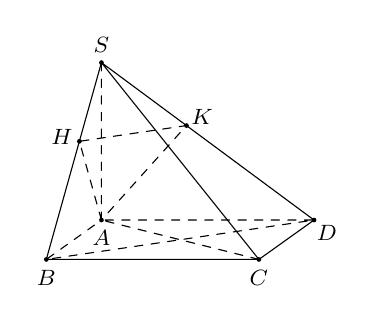
\begin{tikzpicture}[scale=1,>=stealth,font=\footnotesize,line join=round,line cap=round,declare function={h=2;}]
					\path 
						(0,0) coordinate  (A)
						(-0.7,-0.5) coordinate (B) 
						 (2,-0.5) coordinate (C)
						(barycentric cs:A=1,C=1,B=-1) coordinate (D) 
						(A)+(90:h) coordinate (S) 
						(barycentric cs:S=3,B=2) coordinate (H) 
						(barycentric cs:S=3,D=2) coordinate  (K);
					 \draw[dashed] (S)--(A)--(B)
						(C)--(A)--(D)--(B) 
						(A)--(H)--(K)--(A); 
					\draw  (C)--(S)--(B)--(C)--(D)--(S);
					\foreach  \p/\g in{A/-90,B/-90,C/-90,D/-45,S/90,H/165,K/30}
					\fill (\p)  circle (.03) node[shift={(\g:.23)},scale=1]{$\p$};
				\end{tikzpicture}
		\end{center}
		\begin{itemchoice}
			\itemch  $SA\perp(ABCD)$ $\Rightarrow$ $SA\perp BD$.
			\itemch  Nếu $BD\perp(SAC)$ thì $BD\perp AC$. Điều này sai, vì hình chữ nhật hai đường chéo không vuông góc.\\
			 Vậy $BD$ không vuông góc mặt phẳng $(SAC)$.
			\itemch $CD\perp(SAD)$ $\Rightarrow$ $CD\perp AK$.\\ 
			Hơn nữa, $AK\perp SD$ nên  $AK\perp(SAD)$. \hfill $(1)$
			\itemch Từ $(1)$  suy ra $AK\perp SC$. \hfill $(2)$\\
			$BC\perp(SAB)$  $\Rightarrow$ $BC\perp AH$.\\
			Hơn nữa, $AH\perp SB$ nên $AH\perp(SBC)$. Suy ra $AH\perp SC$. \hfill  $(3)$\\
			Từ $(2)$ và $(3)$ suy ra $SC\perp(AHK)$. 
		\end{itemchoice}
	} 
\end{ex}

% nguồn: Ok_dungsai_lop11_Lan2
\begin{ex}%[1H8V2-3]%[ma:b583b8bc]
	Cho hình chóp $S.ABCD$ có đáy là hình thang vuông tại $A$ và $B$ với $AB=BC=a$ và $AD=2a$, cạnh $SA$ vuông góc với mặt phẳng $(ABCD)$.  Gọi $M$ là trung điểm cạnh $AD$.
	\choiceTF 
		{$BD$ vuông góc mặt  phẳng $(SAC)$}
		{\True  $CM$ vuông góc mặt phẳng $(SAD)$}
		{\True Tam  giác $SCD$ vuông tại $C$}
		{Gọi $H$ là trung điểm $SC$. Khi đó, $AH$ vuông góc  cạnh $SD$}
	\loigiai{ 
		\begin{center}
			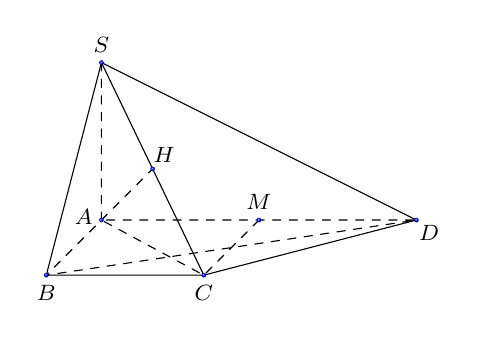
\begin{tikzpicture}[scale=1,>=stealth,font=\footnotesize,line join=round,line cap=round,declare function={h=2;}]
					\path 
						(0,0)  coordinate (A)
						 (-0.7,-0.7) coordinate (B)
						(4,0) coordinate  (D)
						(barycentric cs:A=-1,D=1,B=2) coordinate (C) 
						(A)+(90:h)  coordinate (S)
						(barycentric cs:A=1,D=1) coordinate  (M)
						 (barycentric cs:S=1,C=1) coordinate (H);
					 \draw[dashed] (S)--(A)--(B)
						(M)--(C)--(A)--(D)--(B) 
						 (A)--(H);
					\draw  (C)--(S)--(B)--(C)--(D)--(S);
					\foreach \p/\g in{A/170,B/-90,C/-90,D/-45,S/90,M/90,H/50} 
					\shade[shading=ball](\p) circle (.03) node[shift={(\g:.23)},scale=1]{$\p$}; 
				\end{tikzpicture}
		\end{center}
		\begin{itemchoice}
			\itemch Ta có $M$ là trung điểm cạnh $AD$ và $AD=2a$ nên $AM=a$.  Khi đó, $ABCM$ là hình vuông. Do đó, $BM\perp AC$.\\
			Suy ra  $BD$ không vuông góc với $AC$. Do đó, $BD$ không vuông góc mặt phẳng $(SAC)$.
			\itemch Tứ giác $ABCM$ là hình vuông nên $CM\perp  AD$.\\
			$SA\perp(ABCD)\Rightarrow  CM\perp SA$.\\
			 Vậy $CM\perp(SAD)$.
			\itemch Tam giác $ACD$ có trung tuyến $CM=\dfrac{1}{2}AD$ nên $\triangle ACD$ vuông tại $C$. Suy ra $CD\perp AC$.\\ 
			$SA\perp(ABCD)\Rightarrow CD\perp  SA$.\\
			Suy ra $CD\perp(SAC)$ $\Rightarrow CD\perp  SC$. Do đó, tam giác $SCD$ vuông tại $C$.
			\itemch $CD\perp(SAC)$ và $AH\subset(SAC)\Rightarrow AH\perp  CD$.\\
			Nếu $AH\perp SD$ thì $AH\perp(SCD)$. Khi đó, $AH\perp SC$ nên tam giác $SAC$ cân  tại $A$. Suy ra $SA=AC$ (điều này không có trong giả thiết).\\
			 Vậy $AH$ không vuông góc cạnh $SD$.
		\end{itemchoice}
	} 
\end{ex}

% nguồn: Ok_dungsai_lop11_Lan2
\begin{ex}%[1H8V2-3]%[ma:36a59dc6]
	Cho hình chóp $S.ABC$ có đáy là tam giác $ABC$ vuông tại $B$, cạnh $SA$ vuông góc mặt phẳng $(ABC)$. Gọi  $H$, $K$ lần lượt là hình chiếu vuông góc của điểm $A$ lên cạnh $SB$ và $SC$.
	 \choiceTF
		{\True $SA$ vuông góc  $BC$}
		{$BC$ vuông góc mặt phẳng  $(SAC)$}
		 {\True $SC$ vuông góc mặt phẳng $(AHK)$}
		{Tam giác $AHK$ là  tam giác vuông tại $K$}
	 \loigiai{
		\begin{center}
			\begin{tikzpicture}[scale=1,>=stealth,font=\footnotesize,line join=round,line cap=round,declare function={h=2;}]
					 \path
						(0,0) coordinate  (A)
						(0.7,-0.6) coordinate (B) 
						(2.5,0) coordinate  (C)
						 (A)+(90:h) coordinate (S)
						(barycentric cs:B=2,S=1)  coordinate (H)
						(barycentric cs:C=1,S=2) coordinate (K); 
					 \draw[dashed] (K)--(A)--(C);
					 \draw (K)--(H)--(A)--(B)--(C)--(S)--(A)
						 (S)--(B);
					 \pic[draw,angle radius=4]{right angle=S--H--A};
					\pic[draw,angle  radius=4]{right angle=S--K--A};
					\foreach \p/\g in{A/-135,B/-90,C/-90,S/90,H/0,K/70} 
					\fill  (\p) circle (.03) node[shift={(\g:.23)},scale=1]{$\p$};
				\end{tikzpicture}
		\end{center}
		\begin{itemchoice}
			\itemch $SA\perp(ABC)$ $\Rightarrow$  $SA\perp BC$.
			\itemch $BC\perp(SAC)$  $\Rightarrow$ $BC\perp AC$.
			\itemch $AH\perp(SBC)$  $\Rightarrow$ $AH\perp SC$.\\
			Hơn nữa,  $AK\perp SC$ nên $SC\perp(AHK)$.
			\itemch $AH\perp(SBC)$ và $HK\subset(SBC)$ suy ra  $AH\perp HK$.\\
			Vậy tam  giác $AHK$ vuông tại $H$.
		\end{itemchoice}
	} 
\end{ex}


%%%%%%%%%%%%%%%% TRẢ LỜI NGẮN %%%%%%%%%%%%%%%%

% nguồn: Ok_TraLoiNgan_Lop11_Lan2
\begin{ex}%[1H8H2-3]%[ma:77cc042d]
	Cho hình chóp $S.ABCD$ có đáy $ABCD$ là hình vuông tâm $O$. Biết $SA=SC$ và $SB=SD$, xác định số  đo góc hai đường thẳng $AC$, $SD$. (đơn vị độ)
	\shortans{90} 
	 \loigiai{
	 \immini{
		Ta có $\heva{&AC\perp BD\\&AC\perp  SO}\Rightarrow AC\perp(SBD)\Rightarrow AC\perp SD$.\\
		Vậy $(AC,SD)=90^\circ$. 
		 }
		{\begin{tikzpicture}[line cap=round,line join=round,>=stealth,>=latex,font=\footnotesize,scale=.75]
		\def\a{4} 
		 \def\h{3.5}
		\path  (0:0) coordinate (A)
			++(0:\a) coordinate (D) 
			++(-150:\a/2)  coordinate (C)
			($(A)+(C)-(D)$)  coordinate (B)
			(intersection  of A--C and B--D) coordinate (O)
			($(O)+(90:\h)$) coordinate  (S);
		\draw[dashed] (B)--(A)--(D) 
			 (A)--(S)
			 (A)--(C)
			(B)--(D) 
			(S)--(O); 
		\draw  (B)--(C)--(D)
			(B)--(S) 
			 (C)--(S)
			 (D)--(S);
		\foreach \x/\g in {A/135,B/-135,C/-45,D/45,S/90,O/-90} \fill[black] (\x)  circle (1pt)
			($(\g:3mm)+(\x)$) node  {$\x$};
	\end{tikzpicture}
		 }
	 }
\end{ex}

% nguồn: Ok_TraLoiNgan_Lop11_Lan2
\begin{ex}%[1H8H2-3]%[ma:6bc94f54]
	Cho hình chóp $S.ABCD$ có đáy $ABCD$ là hình vuông và $SA\perp(ABCD)$. Gọi $I$, $J$, $K$ lần lượt là trung điểm của $AB$, $BC$ và $SB$. Xác định góc của hai đường  thẳng $KJ$, $BD$. (đơn vị độ)
	 \shortans{90}
	\loigiai{ 
		\begin{center}
			\begin{tikzpicture}[>=stealth,line join=round,line cap=round,font=\footnotesize,scale=0.7]
					\path (0,0) coordinate (A) 
						(-2.5,-1.4) coordinate (B) 
						 (6,0) coordinate (D)
						($(B)+(D)-(A)$) coordinate  (C)
						 ($(A)+(0,5)$) coordinate (S)
						($(A)!0.5!(C)$) coordinate  (O)
						($(A)!0.5!(B)$) coordinate (I) 
						($(C)!0.5!(B)$) coordinate (J) 
						($(S)!0.5!(B)$) coordinate  (K);
					\draw  (S)--(B)--(C)--(S)--(D)--(C)
						 (K)--(J);
					\draw[dashed] (S)--(A)--(B)--(D)--(A)--(C) 
						 (J)--(I)--(K);
					\foreach \p / \r in {A/135,B/-135,C/-45,S/90,D/45,I/135,J/-90,K/135} 
					 \fill (\p) circle (1pt) node[shift={(\r:2mm)}]{$\p$};
					 \foreach \x/\y/\z in {S/A/D,A/O/B} \draw pic[draw,angle radius=2mm] {right angle= \x--\y--\z};
				\end{tikzpicture}
		\end{center}
		Ta có $\heva{&BD\perp SA\,(\text{do  }SA\perp(ABCD))\\&BD\perp AC\,(ABCD\text{ là hình vuông})}\Rightarrow BD\perp(SAC)$.\hfill $(1)$\\
		Ta có $IK$, $IJ$ lần lượt là đường trung bình của các tam giác $SAB$, $ABC$  nên $IK\parallel SA$, $IJ\parallel AC$.\\
		Suy  ra $(IJK)\parallel (SAC)$.\hfill $(2)$\\
		Từ $(1)$ và  $(2)$, suy ra $BD\perp(IJK)\Rightarrow KJ\perp BD$.\\
		Vậy $(KJ,BD)=90^\circ$. 
	} 
\end{ex}

% nguồn: Ok_TraLoiNgan_Lop11_Lan2
\begin{ex}%[1H8H2-3]%[ma:b76bddcc]
	Cho hình chóp $S.ABC$ có cạnh bên $SA\perp(ABC)$ và đáy $ABC$ là tam giác cân ở $B$. Gọi  $H$ và $K$ lần lượt là trung điểm của $AC$ và $SC$. Xác định góc của hai đường thẳng $BH$, $SC$. (đơn vị độ)\\
	 \shortans{90}
	 \loigiai{
		\begin{center}
			\begin{tikzpicture}
					\def\a{4} 
					\path (0:0)  coordinate (A)
						(0:\a) coordinate (C) 
						(-45:.45*\a) coordinate  (B)
						 ($(A)+(90:\a)$) coordinate (S)
						 ($(A)!0.5!(C)$) coordinate (H)
						($(S)!0.5!(C)$) coordinate (K); 
					\draw  (A)--(B)--(C)
						 (A)--(S)
						(B)--(S) 
						 (C)--(S);
					\draw[dashed]  (A)--(C)
						 (B)--(H)--(K);
					\foreach \x /\goc in {A/180,B/-45,C/0,S/90,K/45,H/-45} 
					\fill[black] (\x) circle (1pt) 
						($(\x)+(\goc:3mm)$) node {$\x$}; 
					\draw pic[draw,angle  radius=2mm]{right angle=C--A--S};
					\draw pic[draw,angle  radius=2mm]{right angle=A--H--B};
				\end{tikzpicture}
		\end{center}
		Tam giác $ABC$  cân tại $B$ có đường trung tuyến $BH$ nên $BH\perp AC$.\hfill $(1)$\\
		 Mặt khác $BH\perp SA$ (do $SA\perp(ABC)$).\hfill $(2)$\\
		Từ $(1)$ và $(2)$  suy ra $BH\perp(SAC)\Rightarrow BH\perp SC$.\\
		Vậy  $(BH,SC)=90^\circ$.
	 }
\end{ex}

% nguồn: Ok_TraLoiNgan_Lop11_Lan2
\begin{ex}%[1H8H2-3]%[ma:9a7ceb4b]
	Cho tứ diện $ABCD$ có $AC=AD$, $BC=BD$. Xác định số đo góc  hai đường thẳng $CD$, $AB$. (đơn vị độ)
	 \shortans{90}
	\loigiai{ 
	\immini{Gọi $I$ là trung điểm của $CD$.\\ 
		Ta có $\heva{&CD\perp BI\\&CD\perp AI}\Rightarrow CD\perp(ABI)\Rightarrow  CD\perp AB$.\\
		Vậy  $(AB,CD)=90^\circ$.
		}{ 
		\begin{tikzpicture}[scale=1,font=\footnotesize,line join=round,line cap=round,>=stealth]
				\path (0,0) coordinate  (B)
					(4,0) coordinate (D) 
					(3,-1.3)  coordinate (C)
					 ($(D)!0.5!(C)$) coordinate (I)
					($(B)!0.6!(I)$) coordinate (H) 
					 ($(H)+(0,2.5)$) coordinate (A);
				 \draw (A)--(B)--(C)--(D)--cycle (I)--(A)--(C);
				\draw[dashed] (I)--(B)--(D); 
				\foreach \p/\g in {B/180,C/-90,D/0,A/90,I/-30} \fill (\p) circle (1pt)+(\g:0.3)  node{$\p$};
				 \foreach \x/\y/\z in {A/I/D,B/I/C} \draw pic[draw,angle radius=0.2cm]{right angle=\x--\y--\z};
			\end{tikzpicture}
		 }
	 }
\end{ex}

% nguồn: Ok_TraLoiNgan_Lop11_Lan2
\begin{ex}%[1H8H2-3]%[ma:aea7229a]
	Cho hình lập phương $ABCD.A'B'C'D'$ có cạnh bằng $a$. Gọi $M$, $N$  lần lượt là trung điểm của $A'B'$, $B'C'$. Góc giữa hai đường thẳng $MN$ và $BD$ là (đơn vị độ)
	 \shortans{90}
	\loigiai{ 
	 \immini{
		 Ta có $MN\parallel AC$ mà $AC\perp BD\Rightarrow MN\perp BD$.\\
		Vậy $(MN,BD)=90^\circ$. 
		}{ 
		\begin{tikzpicture}[line cap=round,line join=round,>=stealth,>=latex,font=\footnotesize,scale=.75]
				\def\h{4} 
				 \path
					(0,0) coordinate (A') 
					(4,0) coordinate  (D')
					(-2,-1) coordinate  (B')
					($(B')+(D')-(A')$) coordinate (C') 
					($(A')+(90:\h)$) coordinate (A) 
					($(B')+(90:\h)$) coordinate (B) 
					($(C')+(90:\h)$) coordinate (C) 
					($(D')+(90:\h)$) coordinate  (D)
					($(B')!.5!(A')$)  coordinate (M)
					($(B')!.5!(C')$) coordinate (N); 
				 \draw (A)--(B)--(C)--(D)--cycle (B)--(B')--(C')--(C)
					 (C')--(D')--(D)
					 (B)--(D)
					 (A)--(C);
				\draw[dashed] (A)--(A') 
					 (B')--(A')--(D')
					 (M)--(N);
				\foreach \x/\g in {A/90,B/180,C/-45,D/0,A'/135,B'/180,C'/-45,D'/0,M/135,N/-90} 
				\fill  (\x) circle (1pt)
					($(\g:3mm)+(\x)$) node  {$\x$};
			\end{tikzpicture}
		 }
	} 
\end{ex}

% nguồn: Ok_TraLoiNgan_Lop11_Lan2
\begin{ex}%[1H8H2-3]%[ma:71eed040]
	Cho hình chóp $S.ABCD$ có đáy là hình vuông $ABCD$ cạnh $a\sqrt{2}$ và $SA=SD=a$. Gọi  $M$ và $N$ lần lượt là trung điểm của $AB$ và $SB$. Số đo góc $(MN,SD)$ bằng (đơn vị độ)
	 \shortans{90}
	 \loigiai{
	\immini{ 
		Ta có $MN$ là đường trung bình của $\triangle  SAB$ nên $MN\parallel SA$.\\
		Suy ra  $(\widehat{MN,SD})=(\widehat{SA,SD})=\widehat{ASD}$.\\
		Xét $\triangle SAD$ có $SA=SD=a$, $AD=a\sqrt{2}$, suy ra  $SA^2+SD^2=AD^2$ nên $\triangle SAD$ vuông tại $S$.\\
		 Vậy $(MN,SD)=90^\circ$.
		 }{
		\begin{tikzpicture}[line cap=round,line join=round,>=stealth,>=latex,font=\footnotesize,scale=.85]
				\def\a{4} 
				\def\h{3.5} 
				\path (0:0) coordinate  (A)
					++(0:\a)  coordinate (D)
					++(-150:\a/2) coordinate (C) 
					($(A)+(C)-(D)$) coordinate  (B)
					(intersection of A--C and B--D) coordinate (O) 
					($(O)+(90:\h)$) coordinate  (S)
					($(S)!.5!(B)$) coordinate  (N)
					($(A)!.5!(B)$)  coordinate (M);
				\draw[dashed]  (B)--(A)--(D)
					(A)--(S) 
					(M)--(N); 
				 \draw (B)--(C)--(D)
					 (B)--(S)
					(C)--(S) 
					 (D)--(S);
				\foreach \x/\g in {A/135,B/-135,C/-45,D/45,S/90,M/-45,N/135} \fill[black]  (\x) circle (1pt)
					($(\g:3mm)+(\x)$)  node {$\x$};
			\end{tikzpicture}
		 }
	 }
\end{ex}

% nguồn: Ok_TraLoiNgan_Lop11_Lan1
\begin{ex}%[1H8V2-3]%[ma:9be07734]
	Cho hình lăng trụ $A B C .A' B' C'$ có đáy là tam giác đều cạnh $a$, $ A' A \perp(A B C)$ và $A' A=2 a$. Gọi $I$ là  trung điểm $B C$. Tính góc giữa hai đường thẳng $A I$ và $B C'$
	 \shortans{90}
	 \loigiai{
		\begin{center}
			\begin{tikzpicture}
					\def\a{3} 
					 \def\h{4}
					\path (0:0)  coordinate (A)
						++(0:\a)  coordinate (C)
						++(-150:3*\a/4)  coordinate (B)
						($(A)+(90:\h)$)  coordinate (A')
						 ($(B)+(90:\h)$) coordinate (B')
						($(C)+(90:\h)$) coordinate  (C')
						 ($(B)!0.5!(C)$) coordinate (I)
						 ($(C')!0.5!(C)$) coordinate (M);
					\draw[dashed]  (I)--(A)--(C)
						 (M)--(A);
					\draw  (C)--(C')--(B)--(B')
						(A)--(A') 
						 (A)--(B)--(C)
						 (M)--(I)
						(A')--(B')--(C')--cycle; 
					\foreach  \x/\g in {A/180,B/-45,C/0,A'/180,B'/-45,C'/0,I/0,M/0}
					\fill[black] (\x) circle  (1pt)
						($(\g:4mm)+(\x)$) node {$\x$}; 
					\draw pic[draw,angle radius=2mm]{right angle=A'--A--B}; 
				\end{tikzpicture}
		\end{center}
		Gọi $M$ là trung điểm $C C'$.\\ 
		Ta có:  $I M \parallel B C' \Rightarrow\left(A I, B C'\right)=(A I, I M)$\\
		Ta có: $A I=\dfrac{a  \sqrt{3}}{2}; I M=\dfrac{1}{2} B C'=\dfrac{1}{2} \sqrt{a^2+(2 a)^2}=\dfrac{\sqrt{5}}{2} a; A M=\sqrt{a^2+a^2}=\sqrt{2} a$\\
		Xét $\triangle A I M$ có: $A M^2=A I^2+I M^2$ nên $\triangle A  I M$ vuông tại $I$. Vậy $(A I, B C)=90^{\circ}$.
	} 
\end{ex}

% nguồn: Ok_TraLoiNgan_Lop11_Lan1
\begin{ex}%[1H8V2-3]%[ma:08e69d08]
	Cho hình chóp  $S. A B C D$ có đáy $A B C D$ là hình vuông. Gọi $H$ là trung điểm của $A B$ và $S H \perp(A B C D)$; gọi $K$ là trung điểm của cạnh $A D$. Xác định góc của hai đường thẳng $A C$ và $S K$ (đơn vị: độ).
	 \shortans{90}
	\loigiai{ 
		\begin{center}
			\begin{tikzpicture}
					\def\a{3} 
					 \def\h{4}
					 \path (0:0) coordinate (A)
						++(0:\a)  coordinate (D)
						++(-130:\a/2)  coordinate (C)
						($(A)+(C)-(D)$) coordinate (B) 
						 ($(A)!0.5!(B)$) coordinate (H)
						($(A)!0.5!(D)$) coordinate  (K)
						 ($(H)+(90:\h)$) coordinate (S)
						 (intersection of A--C and B--D) coordinate (O);
					\draw[dashed] (B)--(A)--(D) 
						 (C)--(A)--(S)
						(S)--(H)--(K)--(S) 
						 (B)--(D);
					 \draw (B)--(C)--(D)
						 (B)--(S)
						 (C)--(S)
						(D)--(S); 
					\foreach \x/\g in {A/135,B/-135,C/-45,D/45,S/90,H/135,K/90} 
					\fill[black] (\x) circle (1pt) 
						($(\g:4mm)+(\x)$)  node {$\x$};
				\end{tikzpicture}
		\end{center}
		Vì $H K$ là đường trung bình của tam giác $A B D$ nên $H K \parallel B D$, mà $B D \perp A C \Rightarrow H K \perp A C$. \hfill{(1)}  \\
		Mặt khác $S H \perp A C \,\,( \text{do }S H \perp(A B C  D))$.\hfill{(2)}\\
		Từ $(1)$ và $(2)$ suy ra $A C  \perp(S H K)$.\\
		Ta lai có $S K \subset(S H K)$ nên $A C \perp  S K$ hay $(A C, S K)=90^{\circ}$.
	 }
\end{ex}

% nguồn: Ok_TraLoiNgan_Lop11_Lan1
\begin{ex}%[1H8V2-3]%[ma:3f123080]
	Cho hình chóp $S.A B C D$ có đáy $A B C D$ là hình vuông và $S A \perp(A B C D)$. Gọi $I, J, K$ lần lượt là trung điểm của $A B$, $B C$ và  $S B$. Xác định góc của hai đường thẳng $K J, B D$ (đơn vị: độ).
	\shortans{90} 
	 \loigiai{
		\begin{center}
			\begin{tikzpicture}
					\def\a{3.5} 
					 \def\h{2.5}
					\path (0:0)  coordinate (A)
						++(0:\a) coordinate  (D)
						 ++(-130:\a/2) coordinate (C)
						($(A)+(C)-(D)$) coordinate (B) 
						 ($(A)+(90:\h)$) coordinate (S)
						 (intersection of A--C and B--D) coordinate (O)
						($(A)!0.5!(B)$)  coordinate (I)
						($(B)!0.5!(C)$)  coordinate (J)
						($(S)!0.5!(B)$) coordinate  (K);
					 \draw[dashed] (B)--(A)--(D)--(B)
						 (A)--(S)
						 (A)--(C)
						(K)--(I)--(J)--(K); 
					\draw (B)-- (C)--(D) 
						(B)--(S) 
						(C)--(S) 
						 (D)--(S);
					\foreach \x/\g  in {A/135,B/-135,C/-45,D/45,S/90,I/120,J/-90,K/180}
					\fill[black] (\x)  circle (1pt)
						($(\g:3mm)+(\x)$)  node {$\x$};
					 \draw pic[draw,angle radius=2mm]{right angle=D--A--S};
					\draw  pic[draw,angle radius=2mm]{right angle=B--A--C};
				\end{tikzpicture}
		\end{center}
		Vì $S A \perp(A B C D)$ nên hình chiếu của $S C$ lên mặt phẳng $(A B C D)$ là $A C$, mà $B D \perp  A C$ nên $B D \perp S C$.\\
		Từ đó, ta có $B D \perp(S  A C)$.\\
		Ta có $I K, I J$ lần lượt là đường  trung bình của các tam giác $S A B, A B C$ nên $I K \parallel S A, I J \parallel A C$.\\
		Suy ra  $(I J K) \parallel(S A C)$.\\
		Khi đó: $\heva{&(I J K) \parallel(S A C) \\ &B D \perp(S  A C)} \Rightarrow B D \perp(I J K)$\\
		mà $K J \subset(I J  K)$ nên $K J \perp B D$.
	} 
\end{ex}

% nguồn: Ok_TraLoiNgan_Lop11_Lan1
\begin{ex}%[1H8V2-3]%[ma:b97d6905]
	Cho hình chóp $S. A B  C D$ có cạnh bên $S A \perp(A B C)$ và đáy $A B C$ là tam giác cân ở $B$. Gọi $H$ và $K$ lần lượt là trung điểm của $A C$ và $S C$. Xác định góc của hai đường thẳng $B H, S C$ (đơn vị: độ).
	\shortans{90} 
	\loigiai{ 
		\begin{center}
			\begin{tikzpicture}
					\def\a{3} 
					\def\h{3} 
					\path (0:0) coordinate  (A)
						++(0:\a) coordinate (C) 
						++(-150:4*\a/5) coordinate  (B)
						($(A)+(90:\h)$) coordinate (S) 
						($(S)!0.5!(C)$) coordinate  (K)
						($(A)!0.5!(C)$) coordinate  (H);
					\draw  (A)--(B)--(C)
						 (A)--(S)
						(C)--(S) 
						 (B)--(S);
					\draw[dashed]  (A)--(C)
						(B)--(H)--(K); 
					\foreach \x /\goc in  {A/180,C/0,B/-135,S/90,H/45,K/20}
					\fill[black] (\x)  circle (1pt)
						($(\x)+(\goc:3mm)$) node {$\x$}; 
					\draw pic[draw,angle radius=2mm]{right angle=C--A--S}; 
				\end{tikzpicture}
		\end{center}
		Tam giác $A  B C$ cân tại $B$ có đường trung tuyến $B H$ nên $B H \perp A C$. \hfill{(1)}\\
		Mặt khác $B H \perp S A  \,\,( \text{do }S A \perp(A B C)$). \hfill{(2)}\\
		Từ $(1)$ và $(2)$ suy ra $B H \perp(S A C)$,  mà $S C \subset(S A C)$ nên $B H \perp S C$.
	 }
\end{ex}

% nguồn: Ok_TraLoiNgan_Lop11_Lan1
\begin{ex}%[1H8V2-3]%[ma:2d5aba10]
	Hình chóp $S.A B C D$ có cạnh $S A$ vuông góc với mặt phẳng $(A B C D)$ và đáy $A B C D$ là hình thang vuông tại $A$ và $D$ với $A  D=C D=\dfrac{A B}{2}$. Xác định góc tạo bời hai đường thẳng $SC$ và $BC$ (đơn vị: độ).
	\shortans{90} 
	\loigiai{ 
		\begin{center}
			\begin{tikzpicture}
					 \def\a{5}
					 \def\h{3}
					\path (0:0)  coordinate (A)
						++(0:\a)  coordinate (B)
						 ($(A)+(-130:\a/2)$) coordinate (D)
						($(B)+(D)-(A)$)  coordinate (Ct)
						 ($(D)!1/2!(Ct)$) coordinate (C)
						($(A)!1/2!(B)$) coordinate (I) 
						($(A)+(90:\h)$) coordinate (S) 
						(intersection of  A--C and B--D) coordinate (O);
					\draw[dashed]  (B)--(A)--(D)
						 (A)--(S)
						 (I)--(C)--(A);
					\draw  (B)--(C)--(D)
						(B)--(S) 
						(C)--(S) 
						(D)--(S); 
					 \foreach \x/\g in {A/135,B/45,C/-45,D/-135,S/90,I/90}
					\fill[black]  (\x) circle (1pt)
						($(\g:3mm)+(\x)$) node {$\x$}; 
					\draw pic[draw,angle  radius=2mm]{right angle=B--A--S};
				\end{tikzpicture}
		\end{center}
		Do $S A \perp(A B C D) \Rightarrow \triangle S A D, \triangle S A B$ vuông tại  $A$.\\
		Gọi  $I$ là trung điểm của $AB$\\
		Xét $\triangle A C B$ có trung tuyyến $C I=\dfrac{1}{2} A  B \Rightarrow \triangle A C B$ vuông tại $C \Rightarrow B C \perp A C$.\\
		Mặt khác  $B C \perp S A \Rightarrow B C \perp(S A C) \Rightarrow B C \perp S C \Rightarrow \triangle S C B$ vuông tại $C \\ \Rightarrow (SC,BC)=90^\circ$.
	 }
\end{ex}

% nguồn: Ok_TraLoiNgan_Lop11_Lan2
\begin{ex}%[1H8V2-3]%[ma:97bbba9e]
	Cho hình lăng trụ $ABC.A'B'C'$ có đáy là  tam giác đều cạnh $a$, $A'A\perp(ABC)$ và $A'A=2a$. Gọi $I$ là trung điểm $BC$. Tính góc giữa hai đường thẳng $AI$ và $BC'$. (đơn vị độ)
	 \shortans{90}
	\loigiai{ 
		\begin{center}
			\begin{tikzpicture}[scale=1,font=\footnotesize,line join=round,line cap=round,>=stealth]
					 \path
						(0,0)  coordinate (A)
						(2,-1.5) coordinate  (B)
						(4,0) coordinate (C) 
						 ($(A)+(0,3)$) coordinate (A')
						 ($(B)+(0,3)$) coordinate (B')
						($(C)+(0,3)$) coordinate  (C')
						 ($(C)!.5!(B)$) coordinate (I)
						($(C)!.5!(C')$) coordinate  (M);
					\draw  (A)--(B)--(C)--(C')--(A')--cycle (A')--(B')
						(B')--(C') 
						 (B')--(B)
						 (M)--(I);
					\draw[dashed] (A)--(C) 
						 (I)--(A)--(M);
					\foreach \i/\g in {A/180,B/-90,C/0,A'/180,B'/-45,C'/0,I/-45,M/0}{\draw[fill=black](\i) circle  (1pt)
						($(\i)+(\g:3mm)$) node{$\i$};} 
					\draw pic[draw,angle radius=3mm]  {angle = M--I--A};
				\end{tikzpicture}
		\end{center}
		Gọi $M$ là trung  điểm $CC'$.\\
		Ta có $IM\parallel BC'\Rightarrow\left(AI,BC'\right)=(AI,IM)$\\ 
		Ta  có
		\begin{itemize}
			\item  $AI=\dfrac{a\sqrt{3}}{2}$.
			 \item $IM=\dfrac{1}{2}BC'=\dfrac{1}{2}\sqrt{a^2+(2a)^2}=\dfrac{\sqrt{5}}{2}a$.
			\item  $AM=\sqrt{a^2+a^2}=\sqrt{2}a$.
		\end{itemize}
		Xét $\triangle AIM$  có $AM^2=AI^2+IM^2$ nên $\triangle AIM$ vuông tại $I$.\\
		 Vậy $\left(AI,BC'\right)=90^\circ$.\\
	 }
\end{ex}

% nguồn: Ok_TraLoiNgan_Lop11_Lan2
\begin{ex}%[1H8V2-3]%[ma:3ad50e3b]
	Cho hình hộp $ABCD.A'B'C'D'$ có  $6$ mặt đều là hình vuông. Gọi $M$, $N$ lần lượt hai điểm tùy ý thuộc hai đoạn thẳng $DD'$, $B'D'$. Xác định số đo góc hai đường thẳng $AC$, $MN$. (đơn vị độ)
	 \shortans{90}
	\loigiai{ 
	 \immini{
		Ta có  $\heva{&B'B\perp AB\\&BB'\perp BC}\Rightarrow BB'\perp(ABCD)\Rightarrow BB'\perp AC$.\\
		Ta có $\heva{&AC\perp BD\\&AC\perp  BB'}\Rightarrow AC\perp\left(BB'D'D\right)\Rightarrow AC\perp MN$.\\
		Vậy  $(AC,MN)=90^\circ$.
		 }
		{ 
		\begin{tikzpicture}
				\def\a{3.5} 
				 \path (0:0) coordinate (A)
					++(0:\a) coordinate  (D)
					++(-130:\a/2)  coordinate (C)
					 ($(A)+(C)-(D)$) coordinate (B)
					($(A)+(90:\a)$) coordinate (A') 
					($(B)+(90:\a)$)  coordinate (B')
					 ($(C)+(90:\a)$) coordinate (C')
					($(D)+(90:\a)$)  coordinate (D')
					($(B')!.7!(D')$)  coordinate (N)
					($(D)!.4!(D')$) coordinate  (M);
				\draw[dashed] (B)--(A)--(D) 
					(A)--(A') 
					(A)--(C) 
					(M)--(N) 
					(B)--(D); 
				\draw (C)--(C') 
					 (D)--(D')
					(B)--(B') 
					 (B)--(C)--(D)
					(A')--(B')--(C')--(D')--cycle  (B')--(D');
				 \foreach \x/\g in {A/180,B/180,C'/135,D/0,A'/180,B'/180,C/-45,D'/0,N/160,M/0}
				\fill[black] (\x)  circle (1pt)
					($(\g:4mm)+(\x)$) node  {$\x$};
			\end{tikzpicture}
		} 
	 }
\end{ex}


%%%%%%%%%%%%%%%% TỰ LUẬN %%%%%%%%%%%%%%%%

% nguồn: Ok_TuanLuan_Toan11_Lan2
\begin{ex}%[1H8H2-3]%[ma:ce1ced46]
	Cho hình chóp $S.ABCD$ có đáy $ABCD$ là hình thang vuông tại $A$ và $B$, $SA\perp (ABCD)$, $AD=2a$, $AB=BC=a$. Chứng minh  rằng $CD\perp SC$.
	 \loigiai{
	\immini{ 
		 Ta có $\heva{& SA\perp (ABCD)\\& CD\subset (ABCD)} \Rightarrow SA\perp CD$. \hfill (1)\\
		Gọi $I$ là trung  điểm của $AD$.\\
		Do tứ giác $ABCI$ là hình vuông nên  $\widehat{ACI}=45^\circ$.\\
		Mặt khác, $\triangle CID$ vuông cân tại $I$  nên $\widehat{DCI}=45^\circ$.\\
		Suy ra $\widehat{ACD}=90^\circ$  hay $AC\perp CD$. \hfill (2)\\
		Từ $(1)$ và $(2)$  suy ra $CD\perp (SAC) \Rightarrow CD\perp SC$.
		 }{
		\begin{tikzpicture}[scale=0.7,font=\footnotesize,line join=round,line cap=round,>=stealth]
				 \def\bc{2.5}
				 \def\ba{2.2}
				\def\ad{5} 
				 \def\h{3}
				\def\gocB{60} 
				\coordinate[label=below:$B$] (B) at (0,0); 
				\coordinate[label=below:$A$]  (A) at (\gocB:\ba);
				\coordinate[label=below:$C$] (C)  at (\bc,0);
				\coordinate[label=right:$D$] (D) at ($(A)+(0:\ad)$); 
				\coordinate[label=above:$S$] (S) at ($(A)+(90:\h)$); 
				 \coordinate[label=above:$I$] (I) at ($(A)!0.5!(D)$);
				 \draw (S)--(B)--(C)--(D)--cycle (S)--(C);
				 \draw[dashed] (B)--(A)--(D)
					 (S)--(A)--(C)--(I)--cycle;
				\foreach \diem in {A,B,C,D,S,I} \fill (\diem) circle (1pt); 
			\end{tikzpicture}
		} 
	} 
\end{ex}

% nguồn: Ok_TuanLuan_Toan11_Lan2
\begin{ex}%[1H8H2-3]%[ma:02d2ed4b]
	Trong mặt phẳng $(P)$ cho $\triangle BCD$ đều.  Gọi $M$ là trung điểm của $CD$, $G$ là một điểm thuộc đoạn thẳng $BM$. Lấy điểm $A$ nằm ngoài $(P)$ sao cho $G$ là hình chiếu vuông góc của $A$ trên $(P)$. Chứng mình rằng $AB\perp CD$.
	 \loigiai{
	\immini{ 
		Vì $AG\perp (BCD)$ nên $BG$ là hình chiếu vuông góc  của $AB$ trên mặt phẳng $(BCD)$.\\
		Mặt khác theo giả thiết $BG\perp  CD$.\\
		Suy  ra $AB\perp CD$ (theo định lý ba đường vuông góc).
		 }{
		\begin{tikzpicture}[scale=0.7,font=\footnotesize,line join=round,line cap=round,>=stealth]
				\def\bd{5} 
				 \def\bc{2}
				 \def\h{4}
				 \def\gocB{-45}
				\coordinate[label=left:$B$]  (B) at (0,0);
				\coordinate[label=below:$C$]  (C) at (\gocB:\bc);
				\coordinate[label=right:$D$] (D) at  (\bd,0);
				\coordinate[label=below right:$M$] (M) at  ($(C)!0.5!(D)$);
				\coordinate[label=below:$G$] (G) at  ($(B)!2/3!(M)$);
				\coordinate[label=above:$A$] (A) at  ($(G)+(90:\h)$);
				\draw (A)--(B)--(C)--(D)--cycle  (M)--(A)--(C);
				 \draw[dashed] (M)--(B)--(D)
					(A)--(G); 
				\foreach \diem  in {A,B,C,D,G,M} \fill (\diem) circle (1pt);
			\end{tikzpicture}
		 }
	} 
\end{ex}

% nguồn: Ok_TuanLuan_Toan11_Lan2
\begin{ex}%[1H8H2-3]%[ma:55f3ecb8]
	Cho tứ diện $ABCD$ có  $AB=AC$, $DB=DC$. Chứng minh $AD\perp BC$.
	\loigiai{ 
	 \immini{
		 Gọi $H$ là trung điểm của $BC$.\\
		Vì $\triangle ABC$  cân tại $A$ và $\triangle DBC$ cân tại $D$ nên ta có
		$$\heva{&  AH\perp BC\\& DH\perp BC} \Rightarrow BC\perp (ADH) \Rightarrow AD\perp BC.$$
		}{ 
		\begin{tikzpicture}[scale=0.7,font=\footnotesize,line join=round,line cap=round,>=stealth]
				\def\bd{5} 
				\def\bc{2} 
				 \def\h{5}
				\def\gocB{-45} 
				\coordinate[label=left:$B$] (B) at  (0,0);
				\coordinate[label=below:$C$] (C) at  (\gocB:\bc);
				\coordinate[label=right:$D$]  (D) at (\bd,0);
				\coordinate[label=below left:$H$] (H) at  ($(B)!0.5!(C)$);
				\coordinate[label=above:$A$] (A) at ($(C)+(80:\h)$); 
				\draw  (A)--(B)--(C)--(D)--cycle (C)--(A)--(H);
				\draw[dashed] (B)--(D)--(H); 
				\foreach \diem in {A,B,C,D,H} \fill (\diem)  circle (1pt);
			\end{tikzpicture}
		} 
	} 
\end{ex}

% nguồn: Ok_TuanLuan_Toan11_Lan2
\begin{ex}%[1H8H2-3]%[ma:60a07b2a]
	Cho hình chóp $S.ABCD$ có đáy $ABCD$ là hình vuông, cạnh bên $SA$ vuông góc với đáy. Gọi $H$, $K$ lần lượt là hình chiếu của  $A$ lên $SC$, $SD$. Chứng minh $HK\perp SC$.
	 \loigiai{
	 \immini{
		Ta có $CD\perp AD$, $CD\perp SA$.\\ 
		Suy ra $CD\perp (SAD) \Rightarrow  CD\perp AK$.\\
		Mà $AK\perp SD$ nên $AK\perp  (SCD)$.\\
		 Suy ra $AK\perp SC$.\\
		Mặt  khác $AH\perp SC$ nên $SC\perp (AHK)$.\\
		Suy  ra $HK\perp SC$.
		}{ 
		\begin{tikzpicture}[scale=0.7,font=\footnotesize,line join=round,line cap=round,>=stealth]
				 \def\bc{4}
				\def\ba{2.2} 
				\def\h{3} 
				\def\gocB{45} 
				\coordinate[label=below:$B$] (B) at (0,0); 
				\coordinate[label=below:$A$] (A) at  (\gocB:\ba);
				\coordinate[label=below:$C$]  (C) at (\bc,0);
				 \coordinate[label=right:$D$] (D) at ($(A)+(0:\bc)$);
				\coordinate[label=above:$S$] (S) at ($(A)+(90:\h)$); 
				\coordinate[label=right:$H$] (H)  at ($(S)!0.5!(C)$);
				\coordinate[label=above  right:$K$] (K) at ($(S)!2/5!(D)$);
				\draw (S)--(B)--(C)--(D)--cycle  (S)--(C)
					 (H)--(K);
				\draw[dashed]  (B)--(A)--(D)
					(S)--(A) 
					(H)--(A)--(K); 
				\foreach \diem in {A,B,C,D,S,H,K} \fill  (\diem) circle (1pt);
			\end{tikzpicture}
		} 
	} 
\end{ex}

% nguồn: Ok_TuanLuan_Toan11_Lan2
\begin{ex}%[1H8H2-3]%[ma:2471ec48]
	Cho hình chóp $S.ABC$ có đáy $ABC$ là tam giác vuông tại $A$ và có $SA\perp (ABC)$. Chứng minh rằng  $AC\perp SB$.
	 \loigiai{
	 \immini{
		Vì $SA\perp (ABC)$ nên $AB$ là hình chiếu  vuông góc của $SB$ trên mặt phẳng $(ABC)$.\\
		Mặt khác theo giả thiết  ta có $AC\perp AB$.\\
		Suy ra $AC\perp SB$ (theo định lý ba  đường vuông góc).
		 }{
		\begin{tikzpicture}[scale=0.7,font=\footnotesize,line join=round,line cap=round,>=stealth]
				\def\ac{4} 
				\def\ba{2} 
				\def\h{3} 
				 \def\gocA{-135}
				\coordinate[label=left:$A$] (A) at  (0,0);
				\coordinate[label=below:$B$] (B) at  (\gocA:\ba);
				\coordinate[label=right:$C$] (C) at (\ac,0); 
				\coordinate[label=above:$S$]  (S) at ($(A)+(90:\h)$);
				 \draw (S)--(B)--(C)--cycle;
				\draw[dashed]  (A)--(C)
					 (S)--(A)--(B);
				\foreach \diem in {A,B,C,S} \fill (\diem)  circle (1pt);
			\end{tikzpicture}
		} 
	} 
\end{ex}
